In this chapter, we throughly describe the Time Stamped Tries approach
to implement a subsumptive tabling engine. This mechanism was proposed by
Ernie Johnson \textit{et al} \cite{Johnson-99} and is currently implemented in XSB.
It is based on the idea of extending each answer trie node with \textit{timestamp}
information as a means to identify new answers from old answers.

First, we start by describing the algorithms and data structures associated
with the detection of subsuming goals. Next, we explain the data structures
introduced in the answer tries to support subsumption, focusing on answer insertion
and retrieval for subsumed subgoals. Then, we describe the modifications made in the YapTab
tabling engine to support subsumptive tabling. Finally, we compare the performance of
the subsumptive YapTab against XSB, and the variant counterparts.

\section{Finding Subsuming Goals}\label{sec:lookup_subsuming}

Both DTSA and TSTs use a similar method that given a call trie $C$ and a subgoal $G$
is able to find a subgoal $G'$ that subsumes $G$.

The search is performed by recursively backtracking through the call trie $C$, trying
to match the node symbols with sub-terms or symbols from $G$. The process stops
once a leaf node is reached successfully.

A non-variable symbol from $G$ must only match with an identical symbol from $C$ and
these types of unifications are always tried first.
If the current trie symbol is a variable, for example \texttt{X}, on the first occurrence \texttt{X}
is bound to the respective $G$ sub-term
and match succeeds; on the next occurrences of \texttt{X}, the current sub-term from $G$ must
be identical to the term bound to \texttt{X}. Throughout the backtracking process, bound variables are
always tried before unbound variables.

Favoring constant values before variables, results in a mechanism that finds \textit{minimally subsuming calls}.
Also, if there is some variant call $G''$ in $C$, $G''$ is found before any other subgoal. If no variant 
or no subsuming call are found, it is possible to save the trie node to insert a new variant call.
This trie node is where the first backtracking occurred or when the first occurrence of
an already seen $G$ variable that could not be paired to a bound trie variable, and instead
must be bound to an unbound trie variable for the process to continue.
The new variant path is then used to keep information about the subsumed goal state in
the leaf call trie node.

\begin{figure}[ht]
  \centering
    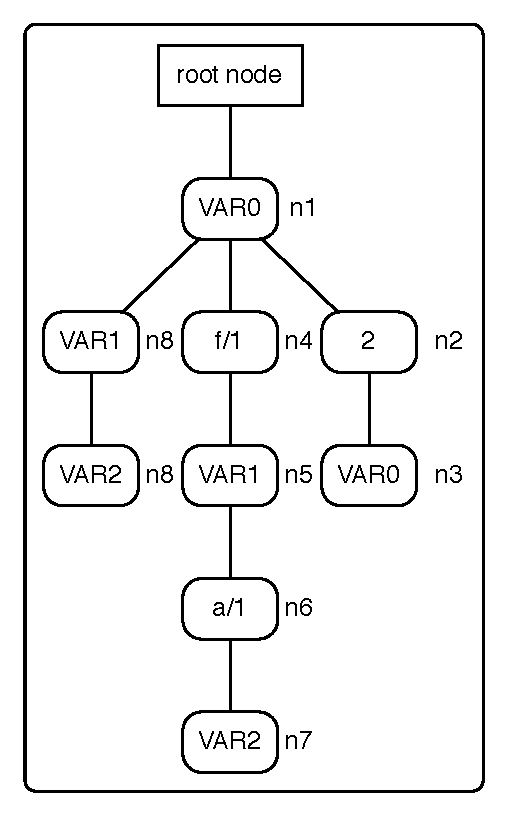
\includegraphics[scale=0.6]{sub_call_search.pdf}
  \caption{Call trie for predicate \texttt{p/3}.}
  \label{fig:sub_call_search}
\end{figure}

For illustration purposes, the Figure \ref{fig:sub_call_search} represents a call trie for the predicate \texttt{p/3}.
The first subgoal called was \texttt{p(X,2,X)}, followed by \texttt{p(X,f(Y),a(Z))} and finally \texttt{p(X,Y,Z)}.

If the subgoal \texttt{p(X,2,X)} is called once again, the algorithm described above
should find the variant subgoal represented by the leaf node $n3$. First, we unify the trie variable
\texttt{VAR0} with \texttt{X} (node $n1$), hence we must also mark the \texttt{X} variable as \textit{seen},
because if the same variable appears again it must unify with the same trie variable for a variant path
to exist. Next, \texttt{2} easily unifies with trie node $n2$ and unification proceeds. In trie node $n3$,
the current call term is \texttt{X} and we also have a variable in the trie node. As \texttt{X} was already seen before,
it must unify with \texttt{VAR0} again, it does and a variant path is found. Please note that if
the trie symbol at node $n3$ was \texttt{VAR1}, the process could proceed but a variant path would be impossible
to exist, and a subsuming subgoal would be found, as \texttt{p(VAR0,2,VAR1)} subsumes \texttt{path(VAR0,2,VAR0)}.
In this case, a variant path could be created by resuming the insert operation at node $n2$ to insert
a \texttt{VAR0} node.

For a more complex example, the subgoal \texttt{p(2,f(X),a(2))} is now called for the same call trie. First,
the algorithm tries to find a trie node with the symbol \texttt{2}, it does not and a variant path
can not be possibly found in this call trie. Next, the algorithm tries to unify with bound variables, but as the process
has just started, only unbound variables can be found and \texttt{VAR0} is unified with \texttt{2} (node $n1$).
The functor term \texttt{f/1} is the next symbol on the subgoal and the first trie node that must be tried is $n4$,
because it contains a non-variable symbol. The next term is \texttt{X} and it can unify with \texttt{VAR1} (node $n5$).
Next, the term symbol \texttt{a/1} matches with trie node $n6$ and the process proceeds. Note that if we failed
at this point, the process would backtrack to node $n2$ and node $n8$ would be tried next, which would
lead to a more general subgoal. Back to node $n6$, the last term symbol \texttt{2} can match with node $n7$, as it is the only trie
node available and it is an unbound variable. If the variable was bound, like \texttt{VAR0} for instance,
the process would check if the current term symbol unifies with the variable binding made before (\texttt{VAR0 = 2}) and
it would also succeed. As node $n7$ is a leaf node, the process finishes and a subsumptive path is found.
The following variable bindings were made: \texttt{VAR0 = 2}, \texttt{VAR1 = X}, and \texttt{VAR2 = 2}.

This algorithm uses various data structures: three auxiliary stacks, a call choice point stack,
a variable bindings vector, and variable enumerator vector. The following summarizes
each data structure: 

\begin{itemize}
  \item \textit{variable bindings vector}: saves bindings for each numbered trie variable. Starts with each position pointing to itself;
  \item \textit{variable enumerator vector}: when a never seen term variable appears it must be bound to a position in this enumerator, ensuring that it can be recognized if it appears a second time;
  \item \textit{term stack}: stores the remaining terms to be unified against trie symbols;
  \item \textit{term log stack}: stores the already matched terms. Each frame contains the top index and the top element of the term stack during frame's creation;
  \item \textit{trail stack}: stores bindings that were made during the process. It is used to untrail variables during backtracking;
  \item \textit{call choice point stack}: used to restore the search process at a certain node to explore alternatives.
\end{itemize}

During execution, two matching methods are considered: the first tries to match exact trie symbols against the current term;
the second method uses trie variables instead of exact symbols and is employed when the first method fails.
When a trie node match succeeds, matching defaults to the first method, which means
that exact matches are always tried before variables when a new \textit{trie level} is reached and variables are mainly
used when backtracking. A trie level represents a set of nodes that are linked by \texttt{sibling} links or are at
the same hash table.

\begin{figure}[ht]
  \centering
    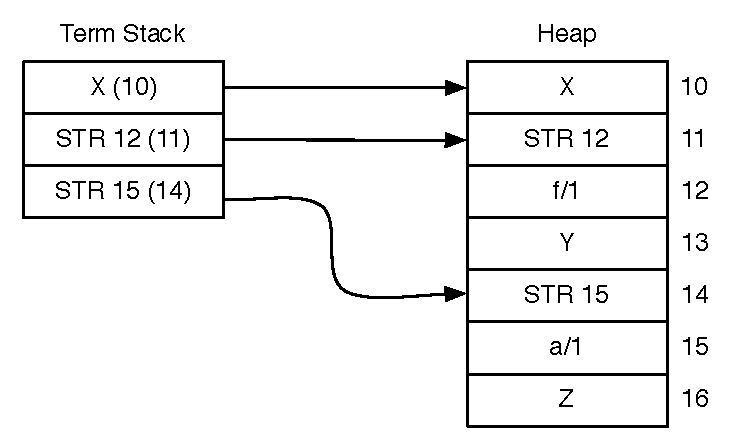
\includegraphics[scale=0.6]{lookup_subgoal_termstack_start.pdf}
  \caption{Initial term stack and heap for subgoal \texttt{p(X,f(Y),a(Z))}.}
  \label{fig:lookup_subgoal_termstack_start}
\end{figure}

The process starts by pushing the $G$ subgoal arguments, $X1, X2, ...Xn$ into the term stack, so that $X1$ is at the top
and $Xn$ at the bottom (Figure \ref{fig:lookup_subgoal_termstack_start}).
Then, the algorithm proceeds in a modified depth-first manner, trying to match the exact nodes first, and then
the variable trie nodes. The skeleton for this algorithm is presented in Figure \ref{fig:lookup_subsuming_call}.

\begin{figure}[ht]
\begin{Verbatim}
lookup_subsuming_call(call_trie, subgoal_call) {
  match_mode = MATCH_EXACTLY
  parent = trie_root(call_trie)
  node = child(parent)
  variable_chain = NULL
  termstack_push_call(subgoal_call)

while_loop:
  while(termstack is not empty) {
    subterm = deref(termstack_pop())
    termstacklog_push(termstack_index(), termstack_top())
  
    if(subterm is atom or integer)
      match_constant(subterm)
    else if(subterm is functor or list)
      match_structured_term(subterm)
    else if(subterm is variable)
      match_variable(subterm)
  
    if(current match failed)
      if(choice point stack is empty) // no more alternatives
        return NO_PATH
      else
        (alt_node, var_chain) = ccpstack_pop_frame()
        match_mode = MATCH_TRIE_VARS
  }
  
  if variant path found
    return (VARIANT_PATH, parent)
  else
    return (SUBSUMPTIVE_PATH, parent)
}
\end{Verbatim}
\caption{Pseudo-code for \texttt{lookup\_subsuming\_call}.}
\label{fig:lookup_subsuming_call}
\end{figure}

\subsection{Call Choice Point Stack}

The call choice point stack (Figure \ref{fig:call_choice_point_stack}) contains alternative
search paths to use if the process fails somewhere in the trie.
Each stack frame can restore the search at a given node by restoring all the auxiliary stacks state at the time
of the call frame creation.

\begin{figure}[ht]
  \centering
    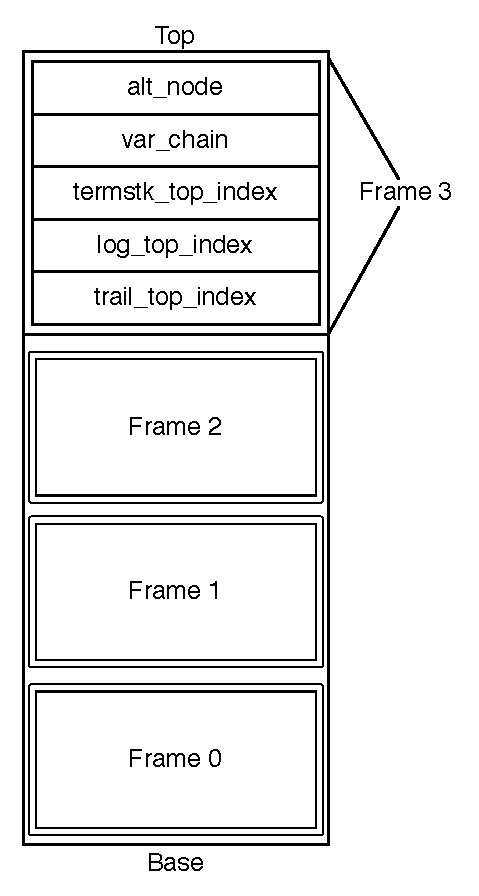
\includegraphics[scale=0.6]{call_choice_point_stack.pdf}
  \caption{Call choice point stack organization.}
  \label{fig:call_choice_point_stack}
\end{figure}

Each frame contains the next trie node to explore (\texttt{alt\_node}),
the current variable chain (\texttt{var\_chain}),
and the following stack indexes during frame creation:
the top of the term stack (\texttt{termstk\_top\_index}),
the top of the term log stack (\texttt{log\_top\_index}),
and the top of the trail stack (\texttt{trail\_top\_index}).
The function \texttt{ccpstack\_push\_frame} (Figure \ref{fig:ccpstack_push_frame})
is used to create a new frame from the computation state.

\begin{figure}[ht]
\begin{Verbatim}
ccpstack_push_frame(alt_node, var_chain) {
  CCPFrame new_frame = new CPPFrame()
  new_frame.alt_node = alt_node
  new_frame.var_chain = var_chain
  new_frame.termstk_top_index = termstack_top - termstack_base + 1
  new_frame.log_top_index = termstacklog_top - termstacklog_base - 1
  new_frame.trail_top_index = trail_top - trail_base
  ccpstack_push(new_frame)
}
\end{Verbatim}
\caption{Pseudo-code for \texttt{ccpstack\_push\_frame}.}
\label{fig:ccpstack_push_frame}
\end{figure}

When popping a frame from the stack, the state of the auxiliary stacks and the other data
structures is restored. Consider a computational state $S1$ that pushed unto the stack
the frame $F1$. Given that we are at state $S2$ and we need to backtrack to the previous state, $S1$,
first we need remove $F1$ from the stack and use the frame's information to restore $S1$.

Any terms that were popped from the term stack from $S1$ to $S2$, which were
stored in the term log stack must be restored back into the term stack.
Then, any bindings made from $S1$ to $S2$ must be untrailed, which is
accomplished by \textit{unwinding} the trail stack. The unwind process untrails
any trie variables bound to the trie variable bindings vector
and any term variable which may have been made to point to the variable enumerator. 

Finally the alternative node and
the variable chain at state $S1$ is also restored. All this is accomplished by the
function \texttt{ccpstack\_pop\_frame} (Figure \ref{fig:ccpstack_pop_frame}).

\begin{figure}[ht]
\begin{Verbatim}
ccpstack_pop_frame() {
  CCPFrame top_frame = ccpstack_pop()
  termstacklog_unwind(top_frame.log_top_index)
  termstack_set_top_of_stack(top_frame.termstk_top_index)
  trail_unwind(top_frame.trail_top_index)
  
  return (top_frame.alt_node, top_frame.var_chain)
}
\end{Verbatim}
\caption{Pseudo-code for \texttt{ccpstack\_push\_frame}.}
\label{fig:ccpstack_pop_frame}
\end{figure}

The node associated with $S2$ and its successors are never visited again and
the process continues until a leaf node is reached or the call choice point stack
is exhausted and the entire trie is visited, yielding no results.

\subsection{Matching Constants}

The \texttt{match\_constant} function is called when the next term from the term stack is a integer or an
atom. First, in phase \textbf{(1)}, the function checks if the match method is to exactly match the
subterm constant against a trie symbol, which means
that this is the first time this trie level is explored. If the current trie level is represented by a simple
linked list, both \texttt{node} and \texttt{var\_chain} point to the start of the chain, but if the trie level
is an hash table, \texttt{node} will point to the symbol bucket and \texttt{var\_chain} to the variable
bucket, which usually is the first bucket.

\begin{figure}[ht]
\begin{Verbatim}
match_constant(constant) {
  if match_mode == MATCH_EXACTLY // (1)
    (node, var_chain) = set_node_and_var_chain(constant)
    match_node = find_matching_node(constant, node)
    if match_node is not NULL
      conditionally_create_choice_point(var_chain)
      descend_node(match_node)
    else // no match found
      node = var_chain
      no_variant_found(parent)
  // no exact match, try bound trie variables (2)
  match_node = find_bound_trie_var(constant, node)
  if match_node is not NULL
    ccpstack_push_frame(next(match_node), var_chain)
    descend_node(match_node)
  // no bound trie variable found, use unbound trie variables (3)
  match_node = find_unbound_trie_var(var_chain)
  if match_node is not NULL
    bind_trie_var(match_node, constant)
    descend_node(match_node)
}
\end{Verbatim}
\caption{Pseudo-code for \texttt{match\_constant}.}
\label{fig:match_constant}
\end{figure}

The function \texttt{find\_matching\_node} iterates a linked list and locates a trie node that contains the
\texttt{constant} symbol. If this node is found we conditionally create a
new choice point (Figure \ref{fig:conditionally_create_choice_point}), that is
we try to find a node with a variable that can be used when backtracking. At this point, only
trie variables can be explored as only one node with the matched symbol exists at this level.

\begin{figure}[ht]
\begin{Verbatim}
conditionally_create_choice_point(var_chain) {
  foreach(node in var_chain)
    if(is_trie_var(node))
      ccpstack_push_frame(node, node)
      return
}
\end{Verbatim}
\caption{Pseudo-code for \texttt{conditionally\_create\_choice\_point}.}
\label{fig:conditionally_create_choice_point}
\end{figure}

Please note that the found variable node is used as the alternative node in this choice point
and as the variable chain, which will be used to try bound and unbound trie nodes, when backtracking happens.

To descend into a node when a matching succeeds the function \texttt{descend\_node} (Figure \ref{fig:descend_node})
is used. It sets the current \texttt{node} and \texttt{parent} information, sets the matching mode for a new trie level
and changes the program flow to the main \texttt{lookup\_subsuming\_call} while loop. But,
if an exact match fails, we know that the current path cannot be variant of the called subgoal, and we call
\texttt{no\_variant\_found} with the parent node as argument.

\begin{figure}[ht]
\begin{Verbatim}
descend_node(target_node) {
  parent = target_node
  node = child(target_node)
  match_mode = MATCH_EXACTLY
  goto while_loop
}
\end{Verbatim}
\caption{Pseudo-code for \texttt{descend\_node}.}
\label{fig:descend_node}
\end{figure}

Phase \textbf{(2)} of \texttt{match\_constant} can be reached by a failed exact match or by backtracking
(remember that the match mode changes to \texttt{MATCH\_TRIE\_VARS} when backtracking). In this step
we call \texttt{find\_bound\_trie\_var} that will iterate over the \texttt{node} chain to look for
\textit{bound trie variables}. When inserting new subgoals on the call trie, each new trie variable
along a path is marked, so it is easy to check for old variables, which have already been bound
to some term before arriving at the current node. The variable binding can be retrieved by
checking the trie variable bindings position for this variable number, which points to an heap term.
Given that we are trying to match a constant symbol, we verify if the bound term matches our symbol.
In this case, we create a new choice point for the sibling node of the matched trie variable, and use
the currently set variable chain.

Finally, if phase \textbf{(1)} and \textbf{(2)} fail, we try to match our constant against an unbound trie variable
(Figure \ref{fig:find_unbound_trie_var}).
Phase \textbf{(3)} can be also reached by a failed exact and bound trie variable match or by subsequent backtrack
attempts. If a node is found, we bind the variable position on the trie variable bindings
vector to point to the new constant. This position is also trailed on the trail stack, so that it can be untrailed
if backtracking is executed.

\begin{figure}[ht]
\begin{Verbatim}
find_unbound_trie_var(var_chain) {
  foreach(node in var_chain)
    if(is_variable(node) and is_new_variable(node))
      return node
}
\end{Verbatim}
\caption{Pseudo-code for \texttt{find\_unbound\_trie\_var}.}
\label{fig:find_unbound_trie_var}
\end{figure}

\subsection{Matching Structured Terms}

When a structured term appears on the term stack, either a functor or a list, the matching process works
just like constants, except the functor or list arguments must be pushed unto the term stack after an exact
match is found (Figure \ref{fig:match_structured_term}).

\begin{figure}[ht]
\begin{Verbatim}
match_structured_term(term) {
  if match_mode == MATCH_EXACTLY // (1)
    (node, var_chain) = set_node_and_var_chain(term)
    match_node = find_matching_node(term, node)
    if match_node is not NULL
      termstack_push_arguments(term)
      conditionally_create_choice_point(var_chain)
      descend_node(match_node)
    else // no match found
      node = var_chain
      no_variant_found(parent)
  // no exact match, try bound trie variables (2)
  match_node = find_bound_trie_var(term, node)
  if match_node is not NULL
    ccpstack_push_frame(next(match_node), var_chain)
    descend_node(match_node)
  // no bound trie variable found, use unbound trie variables (3)
  match_node = find_unbound_trie_var(var_chain)
  if match_node is not NULL
    bind_trie_var(match_node, term)
    descend_node(match_node)
}
\end{Verbatim}
\caption{Pseudo-code for \texttt{match\_structured\_term}.}
\label{fig:match_structured_term}
\end{figure}

Figure \ref{fig:match_functor} shows the evolution of the term stack for finding
a subsuming goal for the subgoal \texttt{p(a,f(b))}. Step \textbf{(1)} shows the initial 
term stack, followed by a match of the term on top of the stack, \texttt{a}, against \textbf{VAR0}.
As it is an unbound trie variable, the first position of the variable bindings vector is
bound to the target term, \texttt{a}.
In step \textbf{(2)}, we try to match the functor \texttt{f/1} against node \textbf{(b)}, but we fail.
Node \textbf{(c)} succeeds as it is an exact match and the functor argument, \texttt{b}, is pushed on
the term stack. In step \textbf{(3)}, \texttt{b} matches against \texttt{b}, and we find a subsuming call:
\texttt{p(VAR0,f(b))}.

\begin{figure}[ht]
  \centering
    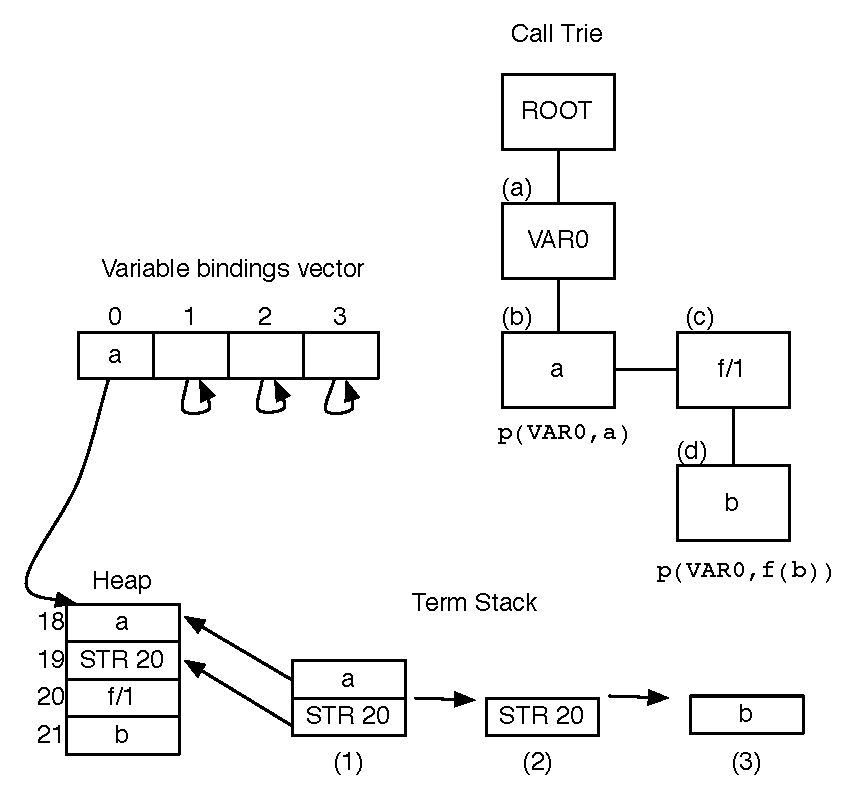
\includegraphics[scale=0.6]{match_functor.pdf}
  \caption{Finding a subsuming goal for subgoal \texttt{p(a,f(b))}.}
  \label{fig:match_functor}
\end{figure}

\subsection{Matching Variables}

The last case for matching terms are variables. Because we are trying to find a more general goal,
a term variable must only be matched or bound against a trie variable and nothing else. More, a
never seen variable must match only with an unbound trie variable, consider the case of trying to
match \texttt{p(X,Y)} against \texttt{p(X,X)}, the first call variable could match the first trie variable,
but the call variable \texttt{Y} must be matched against an unbound variable, thus the next trie variable
(in this case \texttt{VAR0}) cannot be matched, because it was already bound to another variable.
Please note that \texttt{p(X,X)} is subsumed by \texttt{p(X,Y)} and not the other way around.

To recognize already seen call variables, we bind them to the variable enumerator array, indexed
by the corresponding trie variable number and use the trail stack to trail them.
When such call variable must be matched again with a
trie variable, we first try to match it with the same trie variable, and if we fail to find such trie
variable, we use an unbound trie variable, thus, we avoid binding two different call variables to the same
trie variable.

\begin{figure}[ht]
\begin{Verbatim}
match_variable(term) { // term represents a variable on the heap
  if match_mode == MATCH_EXACTLY
    if node is not NULL and is_hash_table(node)
      node = var_chain = hash_bucket(node, VARIABLE_BUCKET)
    else
      var_chain = node
    if variable is not marked(term)
      // variable not seen before
      // only one new trie variable per level, no choice point needed
      foreach(test_node in node) {
        if is_trie_var(test_node) and is_new_variable(test_node)
          bind_trie_var(test_node, term)
          mark_prolog_var(term, var_index(test_node))
          descend_node(test_node)
      no_variant_found(parent)
      backtrack
  // variable has been seen before
  foreach(test_node in node)
    if is_trie_var(test_node) and !is_new_variable(test_node)
      if identical_terms(trie_var_bindings[test_node], term)
        ccpstack_push_frame(next(test_node), var_chain)
        descend_node(test_node)
  // variant path is not possible here
  no_variant_found(parent)
  // match against unbound trie variable
  foreach(test_node in var_chain)
    // only one new trie variable per level, no choice point needed
    if is_trie_var(test_node) and is_new_variable(test_node)
      bind_trie_var(test_node, trie_var_bindings[prolog_var_index(term)])
      descend_node(test_node)
}
\end{Verbatim}
\caption{Pseudo-code for \texttt{match\_variable}.}
\label{fig:match_variable}
\end{figure}

The pseudo-code to match against a variable is displayed in Figure
\ref{fig:match_variable}. From it, we can conclude that a variant path
cannot be found when: (1) a new trie variable cannot be found
for a new call variable, (2) we cannot match an already seen
call variable against the same trie variable already bound to it.

\subsection{Variant Continuations}

The \texttt{lookup\_subsuming\_call} algorithm has the ability to find a
minimally subsuming call and if a variant path exists, it will be found.

A \textit{variant continuation} is built when the algorithm detects that a variant path of the
called subgoal cannot be found on the call trie during the search process.
A variant continuation stores all the needed information to later resume
the algorithm that creates a variant path starting from the last node where the
search for a variant path has failed.

In the above pseudo-code we used the function \texttt{no\_variant\_found} to create
a variant continuation. This function creates a continuation the first time it is called.

The continuation stores the node from where the rest of the variant path is created,
the term stack at creation's time and all the bindings made to the call variables
to the variable enumerator vector that were trailed on the trail stack.

\begin{figure}[ht]
  \centering
    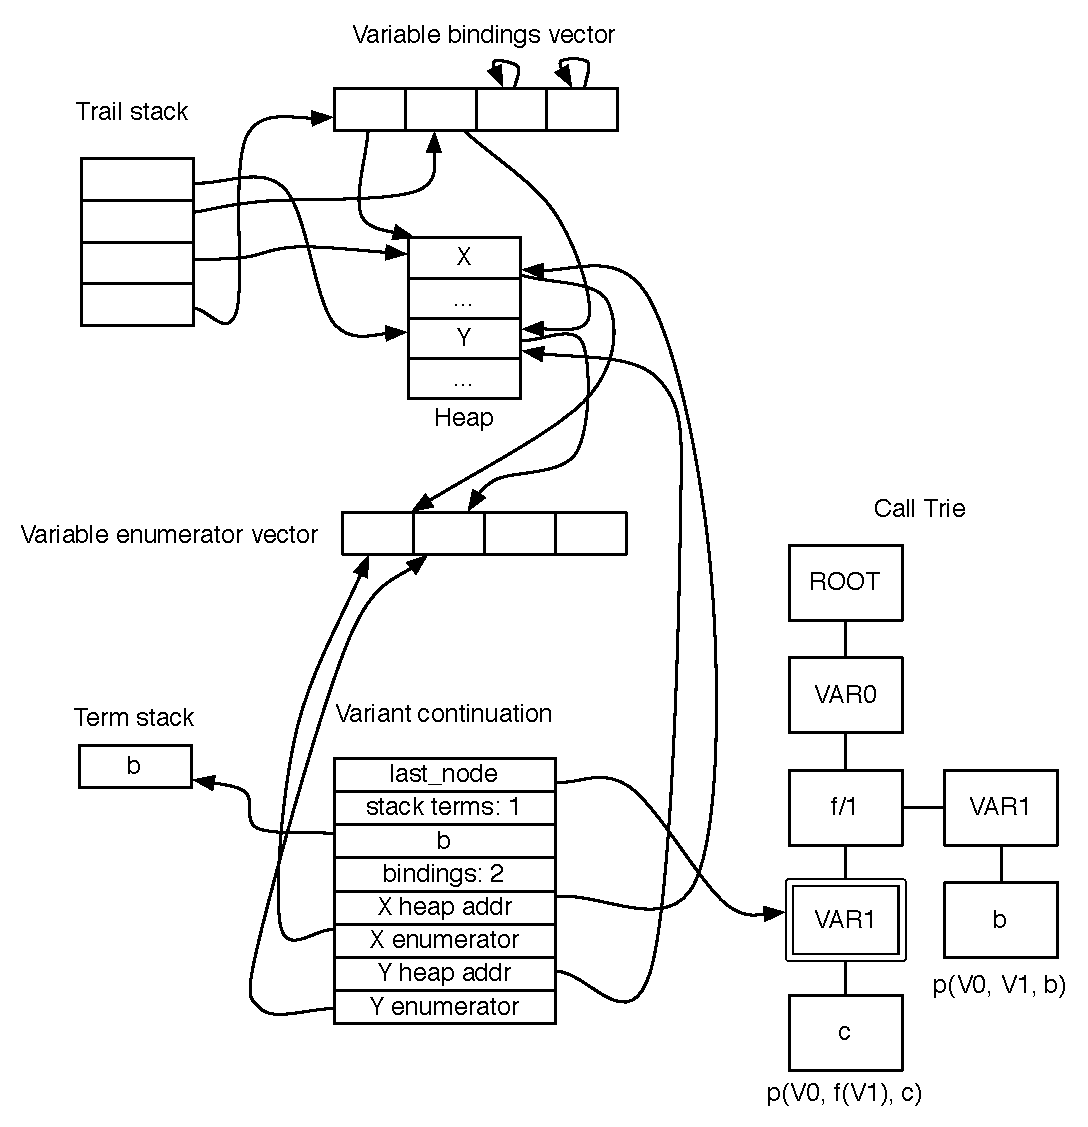
\includegraphics[scale=0.6]{variant_continuation.pdf}
  \caption{Creation of an variant continuation for subgoal \texttt{p(X,f(Y),b)}.}
  \label{fig:variant_continuation}
\end{figure}

Figure \ref{fig:variant_continuation} shows a variant continuation that is built
after the match process failed at node \texttt{c}. If a variant path
for subgoal \texttt{p(X,f(Y),b)} needs to be created: the term stack is restored
with the terms saved on the continuation; the trail stack is initialized with
the two variable heap addresses and each variable is bound to the saved
enumerator addresses. The variable enumerator vector is used during the insertion
of variant paths to detect if a variable was already seen and easily compute its number by
looking at the enumerator position. If it is a new variable, a new trie variable is generated,
and the call variable is pushed on the trail stack and bound to the corresponding enumerator address. 

\section{Answer Templates}

In a variant engine, a substitution factor
represents an array of unique variables which exist in the terms of the argument registers.
These variables are bound to terms when consuming answers from an answer trie.
Figure \ref{fig:answer_template_generator} shows a substitution factor that is constructed
on the local stack below the choice point, in this case a generator choice point.
Note that the substitution factor size (2) is also stored.

\begin{figure}[ht]
  \centering
    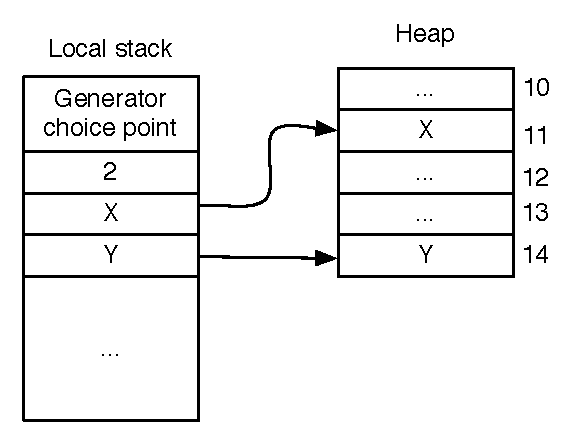
\includegraphics[scale=0.6]{answer_template_generator.pdf}
  \caption{Answer template for generator \texttt{p(X,f(Y))}.}
  \label{fig:answer_template_generator}
\end{figure}

When using call by subsumption, the same factor is used for
subgoals which do not consume from more general subgoals: \textit{generator subgoals}
and variant consumers of generator subgoals.
We call this type of substitution factor a \textit{generator answer template}.

For subgoals with more general subgoals, variants of consumer subgoals and consumers
which consume from consumer subgoals, the answer template must specialize the generator answer template
from the most general subgoal, and is called a \textit{consumer answer template}.
If a generator subgoal \texttt{p(X,f(Y))} exists and the consumer subgoal \texttt{p(a,f(g(2, X)))}
is called, the answer template illustrated on Figure \ref{fig:answer_template_consumer} is built.
Consumer answer templates have the exact same size of generator answer templates
and instead of being composed only of variables, can also be composed with other types of sub-terms.

\begin{figure}[ht]
  \centering
    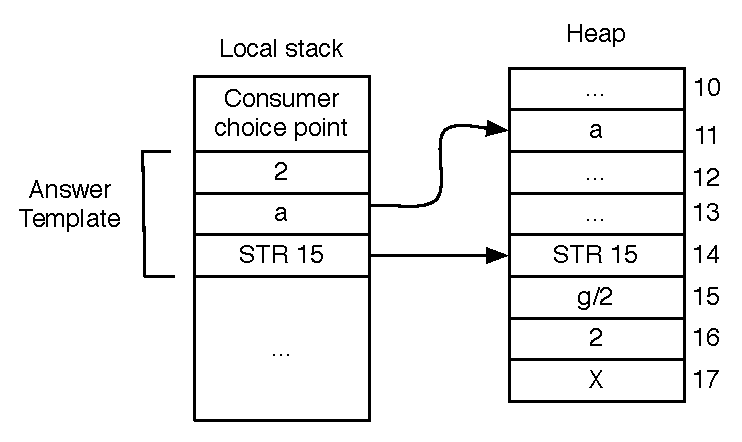
\includegraphics[scale=0.6]{answer_template_consumer.pdf}
  \caption{Answer template for consumer \texttt{p(a,f(g(a,X)))}.}
  \label{fig:answer_template_consumer}
\end{figure}

The construction of answer templates is done when trying to find a general goal on the call trie.
If no subsuming subgoal frame is found, a generator answer template is built. If a subsuming subgoal
is found, the subgoal frame $S$ can be either:

\begin{enumerate}
  \item ... a generator: the answer template is constructed by iterating over the trie variable bindings vector (Figure \ref{fig:extract_template_from_lookup});
  \item ... a consumer: the answer template is reconstructed by using the generator subgoal frame $S'$ from $S$ as we will consume from the generator $S'$ and not $S$. \texttt{reconstruct\_template\_for\_producer} uses another stack, the symbol stack, to push all the trie symbols from the general subgoal path, from leaf to root. The term stack is used to push all the called subgoal arguments that will be matched against the trie symbols. The answer template is then built by matching the new trie variables against the current term on the term stack. Note that when a functor or list symbol appears on the symbol stack the current term is also certainly a functor or list, because the called subgoal specializes the more general subgoal.
\end{enumerate}

\begin{figure}[ht]
\begin{Verbatim}
extract_template_from_lookup(answer_template) {
  total = 0
  foreach(binding in trie variable bindings vector)
    *answer_template-- = binding
    total++
  *answer_template = total
  return answer_template
}
\end{Verbatim}
\caption{Pseudo-code for \texttt{extract\_template\_from\_lookup}.}
\label{fig:extract_template_from_lookup}
\end{figure}

\begin{figure}[ht]
\begin{Verbatim}
reconstruct_template_for_producer(subgoal_call, generator_sf_fr, answer_template) {
  symbol_stack_push_path(leaf_node(generator_sf_fr))
  
  termstack_push_call(subgoal_call)
  
  total = 0
  while(termstack is not empty) {
    subterm = deref(termstack_pop())
    symbol = symbol_stack_pop()
    if is_trie_var(symbol) and is_new_variable(symbol)
      *answer_template-- = subterm
      total++
    else if is_functor(symbol) or is_list(symbol)
      termstack_push_arguments(subterm)
  }
  
  *answer_template = total
  return answer_template
}
\end{Verbatim}
\caption{Pseudo-code for \texttt{reconstruct\_template\_for\_producer}.}
\label{fig:reconstruct_template_for_producer}
\end{figure}

\section{Time Stamped Tries}

A time stamped node extends an answer trie node with timestamp information, thus
each node contains the following fields: \texttt{symbol}, \texttt{child}, \texttt{parent}, \texttt{sibling}
and \texttt{timestamp}. For implementation and algorithmic purposes, each node also needs a bit field,
\texttt{status}, that describes some node properties that will be described shortly.

Insertion of an answer $S$ into a TST can be divided into two phases:

\begin{enumerate}
  \item Finding a more general answer $S'$ on the trie.
  \item Inserting $S$ if $S'$ could not be found.
\end{enumerate}

Step (1) uses the algorithm described in Section \ref{sec:lookup_subsuming} to discover a more general answer, or,
to find a \textit{repeated answer}, which is a variant of $S$.
Step (2) is executed when (1) fails and uses a variant continuation to resume the insertion of the answer
on the last node a variant answer could be found during the search for $S'$.

\begin{figure}[ht]
\begin{Verbatim}
subsumptive_answer_search(trie_root, ans_vector, maintain_tsi)
  (path, leaf) = lookup_subsuming_call(trie_root, ans_vector) // step 1
  if path == NO_PATH
    // step 2
    leaf = tst_insert(trie_root, restore_variant_continuation(), maintain_tsi)
  return leaf
}
\end{Verbatim}
\caption{Pseudo-code for \texttt{subsumptive\_answer\_search}.}
\label{fig:subsumptive_answer_search}
\end{figure}

The function \texttt{subsumptive\_answer\_search} (Figure \ref{fig:subsumptive_answer_search})
implements the two phase process and needs three arguments: the root of the answer trie \texttt{trie\_root},
the answer as a vector of terms \texttt{ans\_vector}, and a boolean argument, \texttt{maintain\_tsi}.

When a chain of sibling nodes becomes larger then a threshold value, we dynamically index the nodes through an hash table to provide direct node access and therefore optimize the search. Given that an hash table
can have a large number of answer nodes, we maintain a double linked list of answer nodes that we keep on the hash
table, in a decreasing order of the time stamp values. This linked list is called a \textit{time stamped index}.
Besides the usual double linked list pointers, each index node contains a pointer to the answer node
and the timestamp for the answer node. Each answer node indexed in the hash table has a different use
for the \texttt{timestamp} field: instead of containing a positive integer, contains a pointer to the respective index node. Figure \ref{fig:hash_table_tst} illustrates an hash table and its time stamp index.

\begin{figure}[ht]
  \centering
    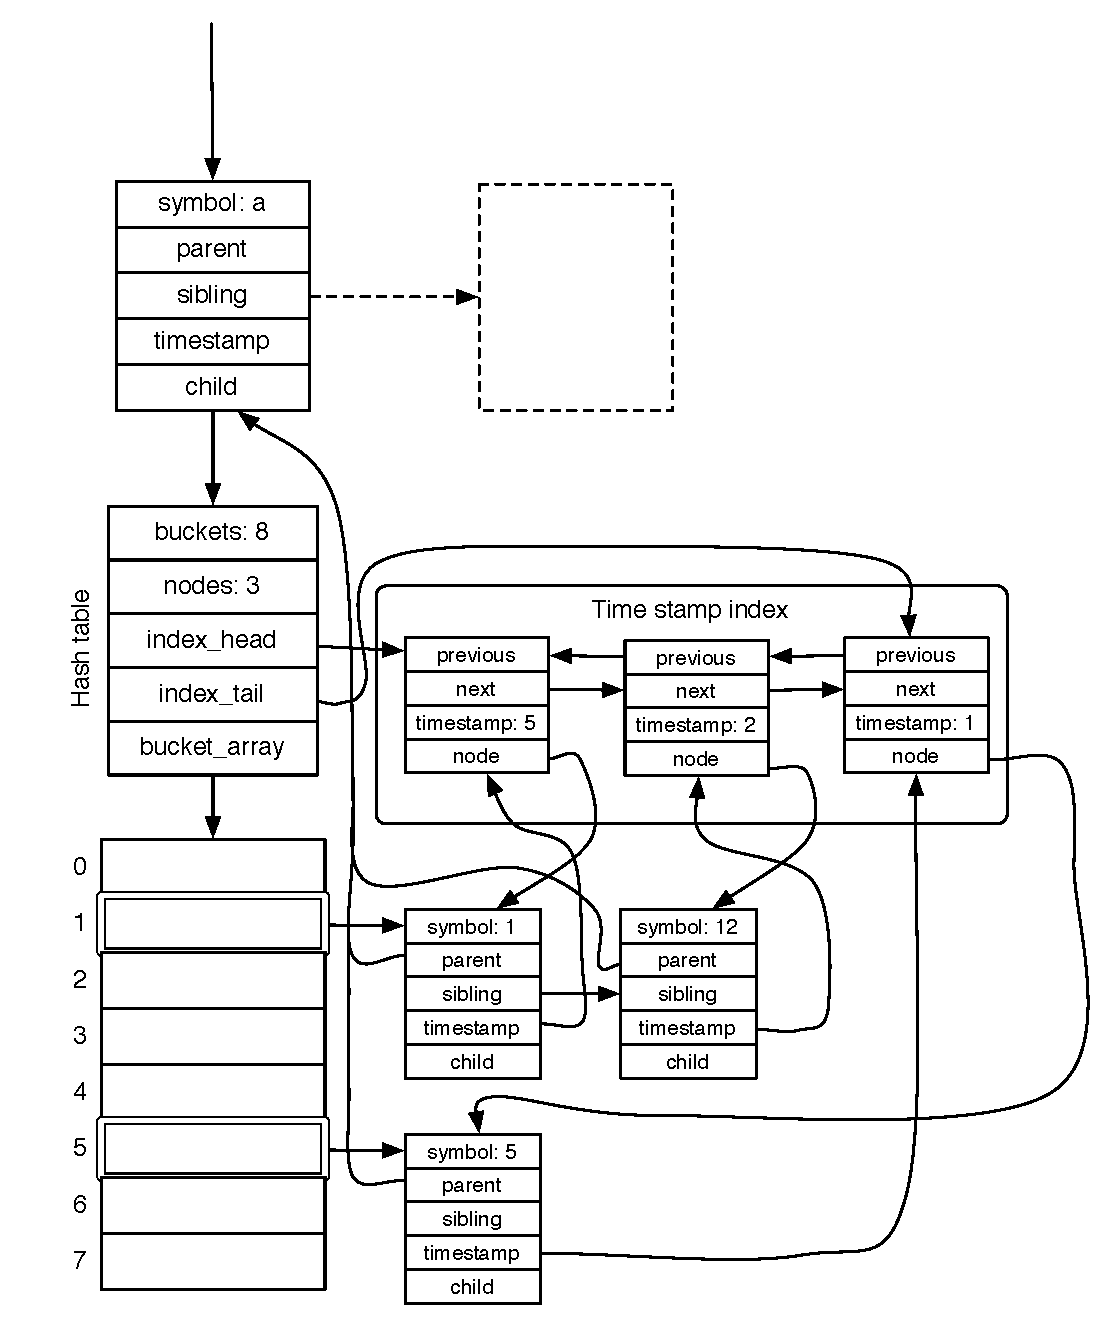
\includegraphics[scale=0.6]{hash_table_tst.pdf}
  \caption{Indexing nodes through an hash table and time stamp indexes.}
  \label{fig:hash_table_tst}
\end{figure}

The argument \texttt{maintain\_tsi} on \texttt{subsumptive\_answer\_search} indicates wether
time stamp indexes exist on the trie and if they need to be maintained.

\subsection{Inserting New Answers}

Once the variant continuation is restored, the rest of the answer path can be inserted on the trie starting
from the restored node. Inserting is then a simple operation because no checking for equal trie symbols is required.
The first symbol will be inserted either: (1) into a childless parent (ie, the trie root); (2) into a node where
we must append the new node in the sibling chain list; (3) into an hashed node, where the symbol must go be indexed.
Every other symbol will be inserted on a childless parent.

\begin{figure}[ht]
\begin{Verbatim}
tst_insert(trie_root, node, maintain_tsi) {
  symbol = process_term_stack()
  if child(node) == null
    // inserting on the root
    node = tst_add_symbol(node, symbol)
  else if is_hash_table(node)
    node = tst_hash_table_add_symbol(node, symbol, maintain_tsi)
  else
    node = tst_insert_symbol(node, symbol, maintain_tsi)
  
  // at this point, just add nodes on childless parents
  while(termstack is not empty) {
    symbol = process_term_stack()
    node = tst_add_symbol(node, symbol)
  }
  
  update_timestamps(node, trie_root, maintain_tsi)
  return node
}
\end{Verbatim}
\caption{Pseudo-code for \texttt{tst\_insert}.}
\label{fig:tst_insert}
\end{figure}

Function \texttt{tst\_insert} (Figure \ref{fig:tst_insert}) does the job of inserting
all the terms contained in a stack of terms into the trie, starting from \texttt{node}.
The difference between functions \texttt{tst\_add\_symbol} and \texttt{tst\_insert\_symbol}
is that the former inserts symbols on childless nodes and the later on nodes with children.

The function \texttt{process\_term\_stack} pops a term from the term stack and converts the term
to a trie representation, which is usually called a \textit{symbol}. If the term is a functor or a list,
the arguments are pushed into the stack of terms, to be processed next.

\begin{figure}[ht]
  \centering
    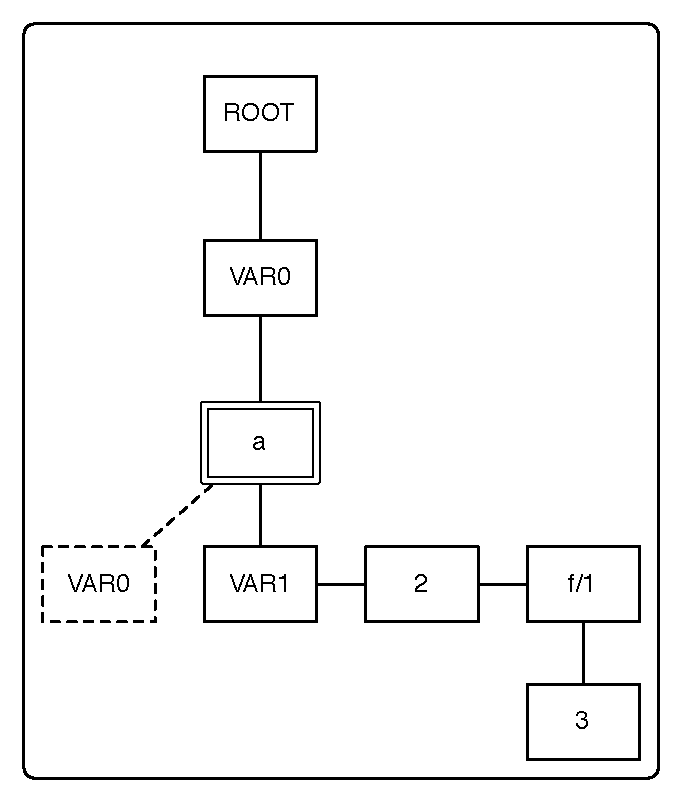
\includegraphics[scale=0.45]{tst_insert.pdf}
  \caption{Inserting answer $\{$\textit{VAR0, a, VAR0}$\}$.}
  \label{fig:tst_chain_insert}
\end{figure}

While appending a new node in a sibling listdoes not involve any
time stamp index (see Figure \ref{fig:tst_chain_insert}), indexing a new node into an hash table does,
because hash tables can index nodes by the time stamp. Figure \ref{fig:hash_table_insert}
illustrates the indexing and insertion of a symbol (25) and the creation of the respective
index node. Note that the \texttt{index head} field was changed to point to the new index node, which
is the node with the greatest time stamp.

\begin{figure}[ht]
  \centering
    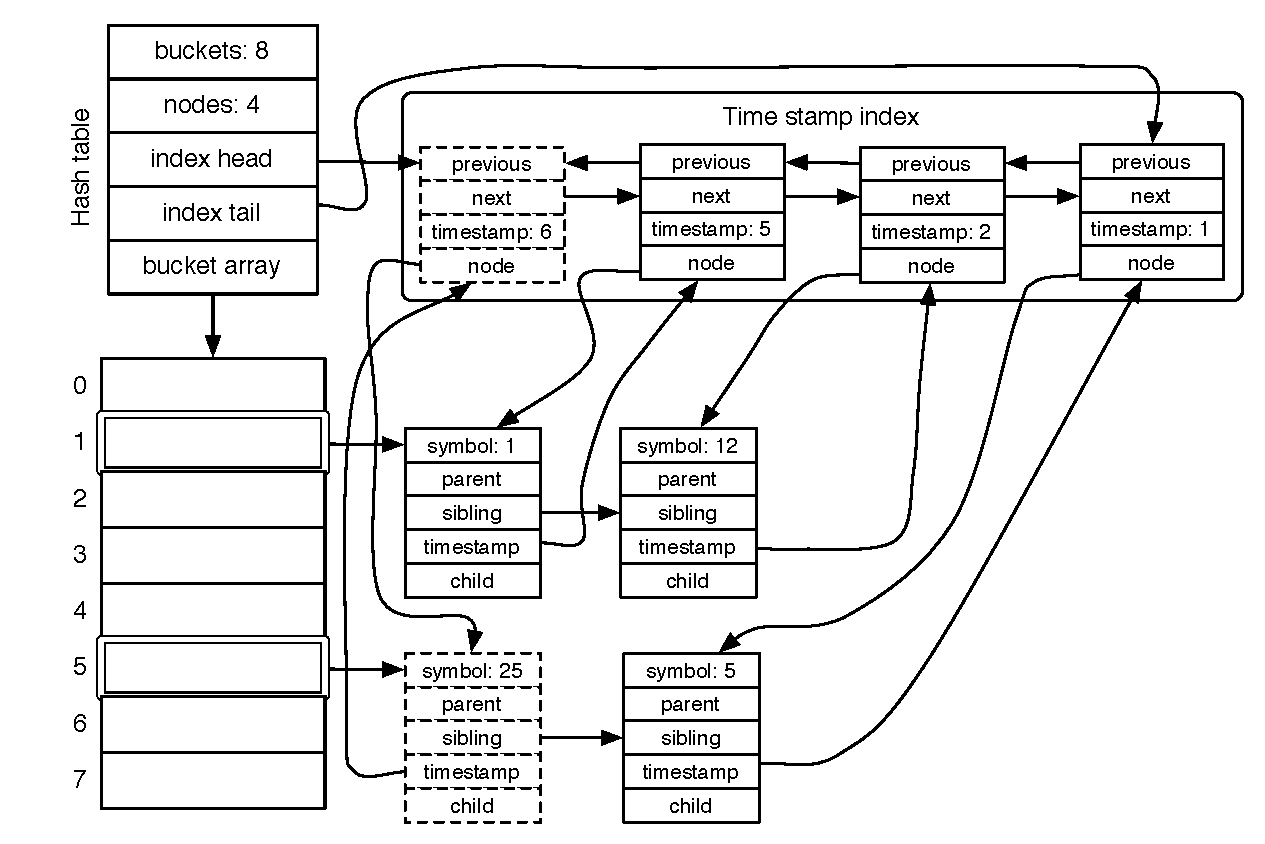
\includegraphics[scale=0.6]{hash_table_insert.pdf}
  \caption{Inserting a node into the hash table and updating the index.}
  \label{fig:hash_table_insert}
\end{figure}

\subsection{Updating Time Stamps}

Once an answer path is inserted, the time stamps must be updated.
The new time stamp is calculated by inspecting the time stamp of the trie root node.
Next, each path node is navigated using the \texttt{parent} field until reaching the root node.

If the current node is an hashed node and the time stamp indexes
must be maintained, its index node is relocated from its position to the head of the index's double linked list. We can test wether an answer node is indexed by an hash table by inspecting
its \texttt{status} field.

Figure \ref{fig:update_timestamps} contains the pseudo-code for the function \texttt{update\_timestamps}.

\begin{figure}[ht]
\begin{Verbatim}
update_timestamps(leaf, root, maintain_tsi) {
  new_timestamp = timestamp(root) + 1
  
  if(maintain_tsi)
    do {
      if is_hashed_node(leaf)
        // relocate index node
        promote_entry(leaf, new_timestamp)
      else
        timestamp(leaf) = new_timestamp
      leaf = parent(leaf)
    } while leaf != root
  else
    do {
      timestamp(leaf) = new_timestamp
      leaf = parent(leaf)
    } while leaf != root
  timestamp(root) = new_timestamp
}
\end{Verbatim}
\caption{Pseudo-code for \texttt{update\_timestamps}.}
\label{fig:update_timestamps}
\end{figure}

When relocating an index node $N$, the \texttt{index head} of the hash table must be modified
to point to $N$. If the $N$ was at the end of the chain,
the field \texttt{index tail} must be updated to the \texttt{previous} field of $N$.
Previous pointers of the \texttt{next} node of $N$ and the next pointer of
the \texttt{previous} node of $N$ must
also be modified to keep the chain consistent.
Figure \ref{fig:hash_table_promote} illustrates the relocation of an index node, during
the time stamp update to 7.

\begin{figure}[ht]
  \centering
    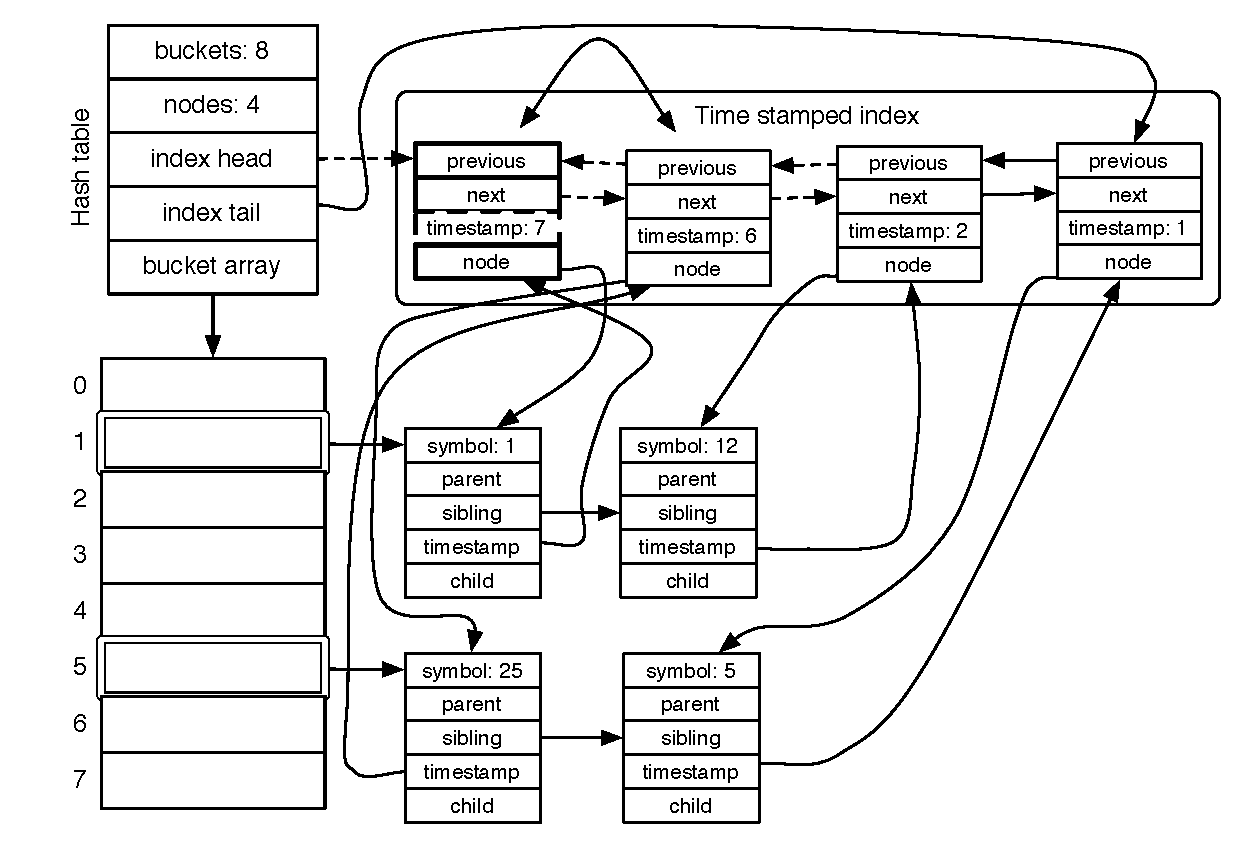
\includegraphics[scale=0.6]{hash_table_promote.pdf}
  \caption{Promoting an index node.}
  \label{fig:hash_table_promote}
\end{figure}

\subsection{Lazy Creation of Time Stamp Indexes}

Time stamped indexes are only maintained when consumer subgoals are first called.
When the first consumer appears, we must iterate over all the hash tables present
on the trie and create the time stamp index.

To efficiently locate all hash tables in an answer trie, we chain these hash tables
with an extra attribute named \texttt{next}. The start of this chain is stored
as the sibling node of the root answer trie node.

Creating the index for an hash table amounts to iterating over the hashed nodes
and orderly inserting new index nodes on the index chain, as it is being created.

When a subgoal completes, the time stamp indexes, which are only used
during collection of relevant answers
for consumer subgoals, are thrown away to save space.

\section{Collecting Relevant Answers}\label{sec:collect}

The process of collecting relevant answers for a consumer subgoal $G$ from an answer trie $T$
of the generator subgoal $G'$, involves searching $T$ for a set $S$ of answers that unify
with the consumer answer template $AT$ and are newer than time stamp
$TS$ stored in the consumer subgoal frame.
When the process ends, $TS$ is updated to the
timestamp of the root node of $T$, thus avoiding repeated answers in future iterations
of the algorithm. Collected answers are also appended into the list of answers of the consumer subgoal frame, so they can be reused in future calls of $G$.

Various data structures are used for this algorithm, namely:

\begin{itemize}
  \item \textbf{WAM data structures}: the push down list (PDL),
  heap, trail, and associated registers. The heap is used to build complex terms, in which the
  answer template or trie variables are bound. Whenever a variable is bound, we trail it using the WAM trail. The \textit{unify} operation provided by the WAM is used to check for term equality in structured terms;
  
  \item \textbf{term stack}: used to store the next terms to be processed as we navigate through the time stamped;
  
  \item \textbf{term log stack}: when an unification fails, there is a need to backtrack to inspect other branch alternatives, this stack is used to store already processed terms of the term stack, so they can be restored back during backtracking;
  
  \item \textbf{variable bindings vector}: stores binds for trie variables;
  
  \item \textit{choice point stack}: stores choice point frames, where each frame is a search alternative and contains information to restore the state of the computation during the frame's creation.
  
\end{itemize}

The pseudo-code for the algorithm is presented in Figure \ref{fig:tst_collect_relevant_answers}.
It starts by pushing the answer template on the term stack, so that the first component to be unified is at the top. Next, we determine the base trail value by comparing TR against the trail freeze register TR\_FZ, this value can then be used to unbind variables before exiting. The trail register is set to the next free position of the WAM trail, thus avoiding writing on frozen segments. Registers HB, H and TR are saved as they will be manipulated and need to be restored to avoid any interference with the normal WAM execution. Answers gathered during execution are maintained in a linked list of trie leafs and are returned once search is over.

The whole algorithm can be summarized into seven steps:

\begin{enumerate}
  \item Fetch a term $T$ from the term stack;
  \item Search for a node $N$ at the current trie level that: (1) has a valid time stamp (2) unifies with $T$;
  \item Search for the next valid node to be pushed on the choice point stack;
  \item Unify $T$ with the trie symbol of $N$;
  \item Proceed into the child of $N$ or, if step 4 fails, backtrack by popping a frame from the choice point stack and use the alternative node to unify;
  \item Once a leaf is reached, mark a new answer and possibly backtrack to retrieve more answers and go to step (1).
  \item If no more choice point frames exist, return the marked answers.
\end{enumerate}

\begin{figure}[ht]
\begin{Verbatim}
tst_collect_relevant_answers(trie_root, ts, answer_template)
{
  answers = new List()
  
  termstack_push_template(answer_template)
  
  // save WAM registers
  trail_base = TR > TR_FZ ? TR : TR_FZ
  saved_HB = HB
  saved_H = HB = H
  saved_TR = TR
  TR = TR > TR_FZ ? TR : TR_FZ
  
  parent = trie_root
  chain = child(parent)
  
while_loop:
  while(termstack is not empty) {
    subterm = deref(termstack_pop())
    
    if(subterm is atom or integer)
      unify_constant(subterm)
    else if(subterm is functor or list)
      unify_structured_term(subterm)
    else if(subterm is variable)
      unify_variable(subterm)
      
    if choice point stack is empty
      unwind_trail(trail_base)
      restore_wam_registers()
      return answers
    
    choice_point_backtrack()
  }
  
  // new relevant answer found
  list_insert_answer(answers, parent)
  
  // no more choice points?
  if choice point stack is empty
    unwind_trail(trail_base)
    restore_wam_registers()
    return answers
    
  choice_point_backtrack()
  goto while_loop
}
\end{Verbatim}
\caption{Pseudo-code for \texttt{tst\_collect\_relevant\_answers}.}
\label{fig:tst_collect_relevant_answers}
\end{figure}

\subsection{Choice Point Stack}

Each choice point frame (Figure \ref{fig:choice_point_stack}) stores the alternative node to explore, the top of the term stack, the top of the term log stack, the current trail position, and the register HB. The HB register serves the same purpose as a WAM choice point saved HB, it is used to store the value of the H register during the choice point creation, so it can restored when backtracking. Figure \ref{fig:cpstack_push_frame} presents pseudo-code for the function \texttt{cpstack\_push\_frame}, which creates a new choice point frame.

\begin{figure}[H]
  \centering
    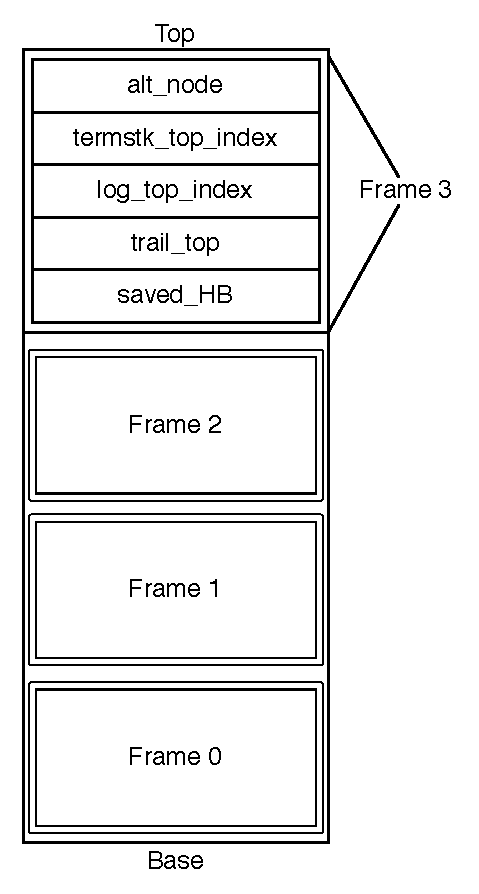
\includegraphics[scale=0.45]{choice_point_stack.pdf}
  \caption{Choice point stack organization.}
  \label{fig:choice_point_stack}
\end{figure}

During execution, the value of the WAM's HB register is compared against the value H to determine if a variable is \textit{conditional}, that is, to determine if a variable needs to be trailed, so that when execution backtracks to a previous choice point we can reset variable bindings. In our case, instead of executing WAM code, we unify a time stamped node, thus the meaning of a conditional variable is extended to include trie variables through the variable bindings vector.

\begin{figure}[h]
\begin{Verbatim}
cpstack_push_frame(alt_node) {
  if alt_node is NULL
    return
  CPFrame frame = new Frame()
  frame.alt_node = alt_node
  frame.termstk_top_index = termstack_top() - termstack_base() + 1
  frame.log_top_index = termstacklog_top() - termstacklog_base()
  frame.trail_top = TR
  frame.saved_HB = H
  cpstack_push(frame)
}
\end{Verbatim}
\caption{Pseudo-code for \texttt{cpstack\_push\_frame}.}
\label{fig:cpstack_push_frame}
\end{figure}

When a choice point frame is popped from the stack (Figure \ref{fig:cpstack_pop_frame}),
the state of the computation is resumed:

\begin{itemize}
  \item the current node and parent node are reset;
  \item all terms stored in the term log stack are pushed into the term stack;
  \item the trail is unwinded to reset variables that existed during the choice point creation and were bound to terms;
  \item registers H and HB are also reseted to previous values.
\end{itemize}

\begin{figure}[h]
\begin{Verbatim}
cpstack_pop_frame() {
  Frame top_frame = cpstack_pop()
  chain = top_frame.alt_node
  parent = parent(chain)
  termstacklog_unwind(top_frame.log_top_index)
  termstack_set_top_of_stack(top_frame.termstk_top_index)
  trail_unwind(top_frame.trail_top)
  H = HB
  HB = top_frame.saved_HB
}
\end{Verbatim}
\caption{Pseudo-code for \texttt{cpstack\_pop\_frame}.}
\label{fig:cpstack_pop_frame}
\end{figure}

\subsection{Constant Unification}

Once a trie node $N$ is reached we must select the next trie node $N'$ that unifies with our term and has a valid time stamp. Node $N$ can lead either to a simple node chain or an hash table.
With constant terms we can index the hash table to prune the search space (\texttt{set\_match\_and\_unify\_chains}) by using the \textit{match bucket}.

\begin{figure}[ht]
\begin{Verbatim}
unify_constant(constant) {
  if is_hash_table(chain)
    // retrieve the indexed and variable buckets
    (chain, alt_chain) = set_match_and_unify_chains(constant)
    if chain != alt_chain
      search_chain_exact_match(chain, constant, ts, alt_chain)
      // exact match failed
      chain = alt_chain
    if chain is NULL
      backtrack
  search_chain_unify_with_constant(chain, constant, ts)
}
\end{Verbatim}
\caption{Pseudo-code for \texttt{unify\_constant}.}
\label{fig:unify_constant}
\end{figure}

Because variables can unify with the constant term, there is the need to retrieve the variable chain (from the variable bucket), which will be used as the alternative chain to push on the choice point stack. We call it the \textit{unify chain}. If the constant is found on the match chain, the unify chain is used as alternative, but if no match was found, the variable chain will be attempted next and, depending on the remaining nodes, also be used as the backtracking alternative.

\begin{figure}[ht]
\begin{Verbatim}
search_chain_exact_match(chain, term, ts, alt_chain) {
  foreach(node in chain) {
    if(term == symbol(node))
      if(valid_timestamp(timestamp(node), ts))
        cpstack_push_frame(chain_next_valid_node(alt_chain, ts))
        termstacklog_push(termstack_index(), termstack_top())
        descend_tst(node)
      else
        return NULL
  }
  return NULL
}
\end{Verbatim}
\caption{Pseudo-code for \texttt{search\_chain\_exact\_match}.}
\label{fig:search_chain_exact_match}
\end{figure}

In Figure \ref{fig:unify_constant} we present the pseudo-code for \texttt{unify\_constant}. Note that we check for an hash table first and inspect the match bucket using \texttt{search\_chain\_exact\_match} (Figure \ref{fig:search_chain_exact_match}).
Finally, if no match is found we set \texttt{chain} to \texttt{alt\_chain} (the unify chain) and execute \texttt{search\_chain\_unify\_with\_constant} on the unify chain. If no hash table was found, we would consider the simple chain of sibling nodes as the unify chain and simply execute \texttt{search\_chain\_unify\_with\_constant}.

\begin{figure}[ht]
\begin{Verbatim}
search_chain_unify_with_constant(chain, constant, ts) {
  chain = chain_next_valid_node(chain, ts)
  while(chain is not null) {
    alt_chain = chain_next_valid_node(sibling(chain), ts)
    symbol = trie_deref(symbol(chain))
    if symbol is variable // case (1)
      cpstack_push_frame(alt_chain)
      bind_and_conditionally_trail(symbol, constant)
      termstacklog_push(constant)
      descend_tst(chain)
    else if symbol == constant // case (2)
      // exact match
      cpstack_push_frame(alt_chain)
      termstacklog_push(constant)
      descend_tst(node)
    else
      chain = alt_chain
  }
  // case (3)
}
\end{Verbatim}
\caption{Pseudo-code for \texttt{search\_chain\_unify\_with\_constant}.}
\label{fig:search_chain_unify_with_constant}
\end{figure}

When using a unify chain, we locate the next node with a valid time stamp on the chain, that is, with the time stamp greater than our target time stamp. Next we "dereference" the node symbol by using
\texttt{trie\_deref}, which returns a position on the variable bindings vector if the node symbol is a trie variable, hence allowing trie variables to be used as "normal" variables.

Please note that the function \texttt{bind\_and\_conditionally\_trail} tests if the variable (first argument) is a conditional variable and then trails it using the WAM trail.

In case (1), a variable was found, which can be a position on the variable bindings vector or a prolog variable that was bound to a trie variable; either way, we bind the variable to the constant term, push a new choice point frame with the next valid node, and descend into the child node of \texttt{chain}.

In case (2) the node symbol matches our constant and we simply push a new choice point frame and advance into the next node.

If we could not found a valid trie node in the unify chain, case (3), the next choice point is popped from the choice point stack and the alternative is tried. If the stack is empty, the algorithm finally ends.

As an example, let's consider the time stamped trie in Figure \ref{fig:collect_example_1}. The input answer template is $\{$\texttt{a,b,b}$\}$ and the target time stamp is 3.

\begin{figure}[H]
  \centering
    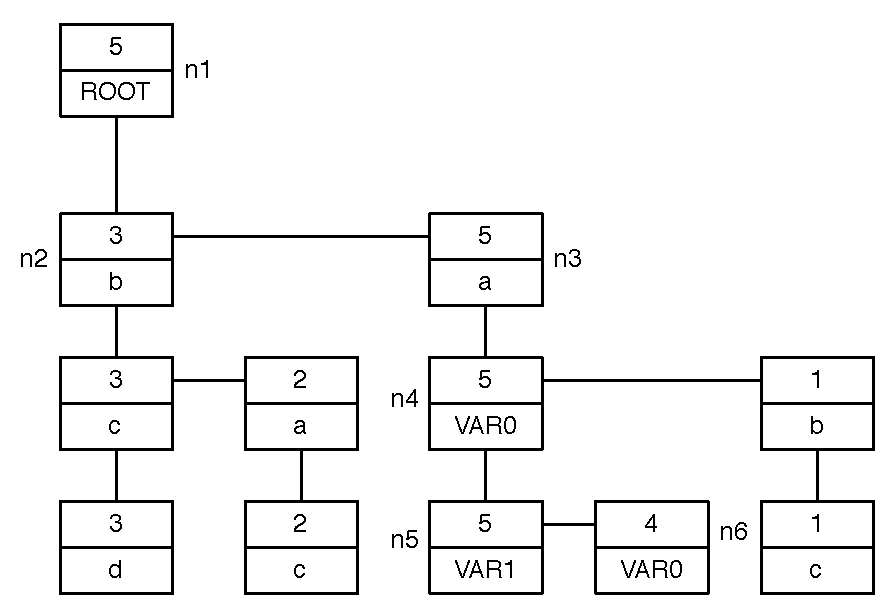
\includegraphics[scale=0.6]{collect_example_1.pdf}
  \caption{Example time stamped trie.}
  \label{fig:collect_example_1}
\end{figure}

We start on node (a) (Figure \ref{fig:collect_ex1}), the root of the trie. The unify chain
is composed by nodes (b) and (c). Node (b) is discarded because the time stamp is invalid.
Node (c) has a valid time stamp and its symbol matches with the current term, \texttt{a}.

\begin{figure}[H]
  \centering
    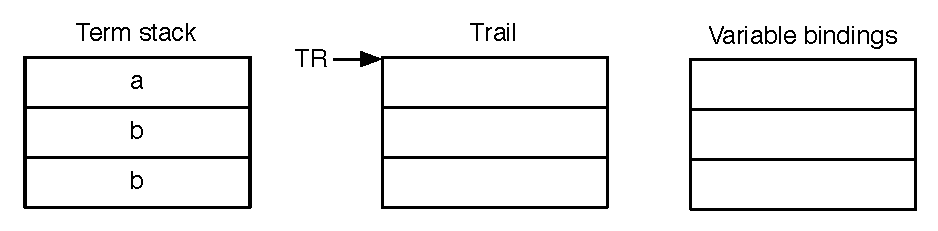
\includegraphics[scale=0.6]{collect_ex1.pdf}
  \caption{At trie node (a).}
  \label{fig:collect_ex1}
\end{figure}

On node (c), our first alternative, node (d) has a valid time stamp and, after doing
\texttt{trie\_deref} we find an unbound variable, \textbf{VAR0}, which is represented
by the first position of the variable bindings vector.
This variable is trailed and bound to \texttt{b},
resulting in what is presented in Figure \ref{fig:collect_ex2}.

\begin{figure}[H]
  \centering
    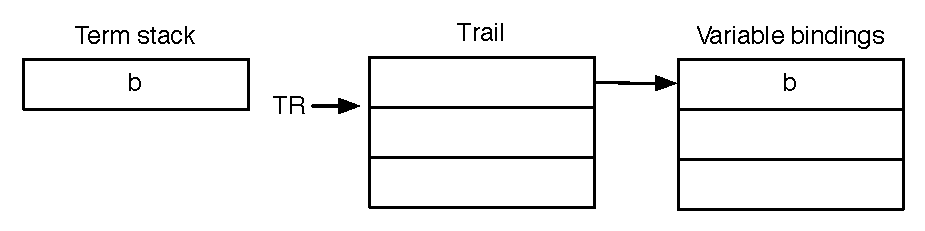
\includegraphics[scale=0.6]{collect_ex2.pdf}
  \caption{At trie node (d).}
  \label{fig:collect_ex2}
\end{figure}

On node (d), the unify chain is composed by nodes (e) and (f). Both have valid time stamps (> 3).
Node (e) is attempted first and easily unifies, because it is an unbound trie variable.
Leaf node (e) is our first answer (Figure \ref{fig:collect_ex3}).

\begin{figure}[H]
  \centering
    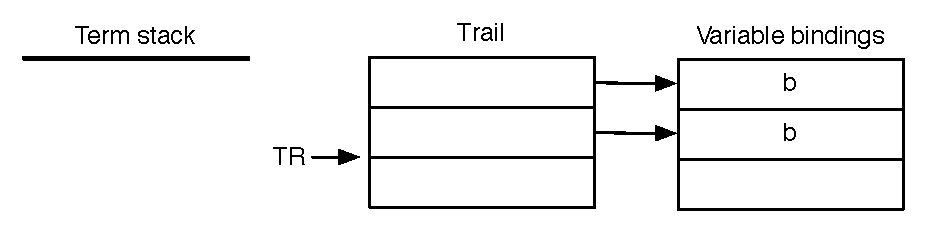
\includegraphics[scale=0.6]{collect_ex3.pdf}
  \caption{At trie node (e).}
  \label{fig:collect_ex3}
\end{figure}

Now, we need to backtrack to collect the other answers. The top choice point frame is retrieved from the stack resulting in a variable being untrailed and the term \texttt{b} being pushed into the term stack (Figure \ref{fig:collect_ex4}).

\begin{figure}[H]
  \centering
    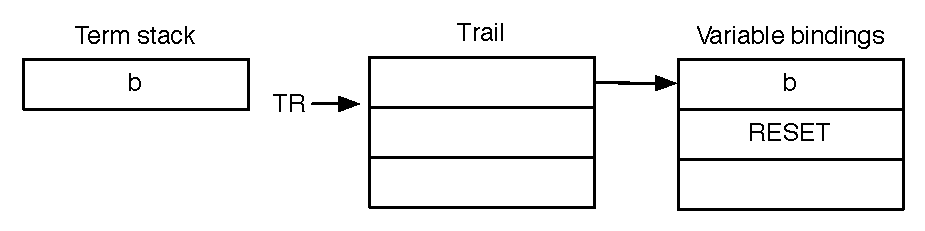
\includegraphics[scale=0.6]{collect_ex4.pdf}
  \caption{Backtracking to node (f).}
  \label{fig:collect_ex4}
\end{figure}

In node (f) we dereference the trie variable \texttt{VAR0} and get the constant term \texttt{b}, which matches the target term. No binding or trailing is needed and we succeed in collecting another relevant answer (Figure \ref{fig:collect_ex5}).

\begin{figure}[H]
  \centering
    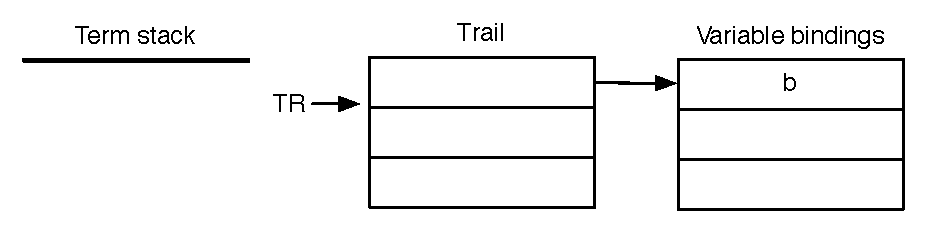
\includegraphics[scale=0.6]{collect_ex5.pdf}
  \caption{New answer as the leaf node (f).}
  \label{fig:collect_ex5}
\end{figure}

As there are no more available choice points we need to untrail any bindings made and return
the answers found (Figure \ref{fig:collect_ex6}), finishing the search.

\begin{figure}[H]
  \centering
    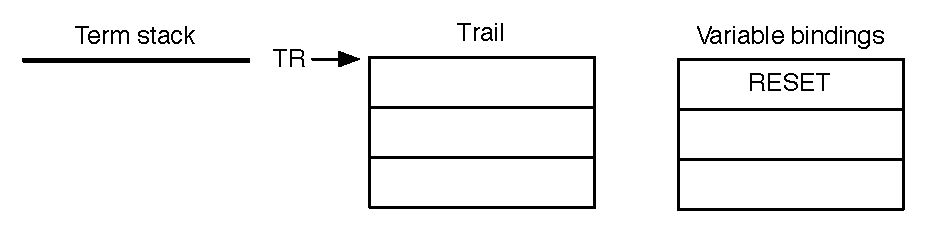
\includegraphics[scale=0.6]{collect_ex6.pdf}
  \caption{Untrailing variables and returning.}
  \label{fig:collect_ex6}
\end{figure}

\subsection{Unification of Structured Terms}

For structured terms, the unification process is similar to constant unification. The
current term in the term stack must be a functor or a list. First, we check if the current
trie node is an hash table and the match and unify chains are computed.
If the match chain contains a valid trie node, before we descend into the child
node we must push the functor or list arguments into the term stack, so they can
be unified with the next trie nodes.

\begin{figure}[ht]
\begin{Verbatim}
unify_structured_term(term) {
  if is_hash_table(chain)
    // retrieve the indexed and variable buckets
    (chain, alt_chain) = set_match_and_unify_chains(term)
    if chain != alt_chain
      search_chain_exact_match_push(chain, term, ts, alt_chain)
      // exact match failed
      chain = alt_chain
    if chain is NULL
      backtrack
  search_chain_unify_with_structured_term(chain, term, ts)
}
\end{Verbatim}
\caption{Pseudo-code for \texttt{unify\_structured\_term}.}
\label{fig:unify_structured_term}
\end{figure}

When using the unify chain with \texttt{search\_chain\_unify\_with\_structured\_term}
\ref{fig:search_chain_unify_with_structured_term},
we also loop the chain for valid time stamped nodes.
Four situations may arise:

\begin{enumerate}
  \item The current term is variable, which is trail and bound to the structured term;
  \item The trie symbol is a structured term and matches our functor or list.
  The term arguments are pushed into the term stack for unification;
  \item We find a trie variable bound to a structured term. The WAM function \texttt{unify} is executed to check for a match and perform additional unifications;
  \item No match was found, the next alternative node is inspected.
\end{enumerate}

\begin{figure}[ht]
\begin{Verbatim}
search_chain_unify_with_structured_term(chain, term, ts) {
  chain = chain_next_valid_node(chain, ts)
  while(chain is not null) {
    alt_chain = chain_next_valid_node(sibling(chain), ts)
    symbol = trie_deref(symbol(chain))
    if symbol is variable // case (1)
      cpstack_push_frame(alt_chain)
      bind_and_conditionally_trail(symbol, term)
      termstacklog_push(term)
      descend_tst(chain)
    else if symbol is a structured term
      if original type of symbol is a structured term and symbol == term
        // case (2)
        cpstack_push_frame(alt_chain)
        termstacklog_push(term)
        termstack_push_arguments(term)
        descend_tst(chain)
      else if unify(term, symbol) // case (3)
        // trie variable bound to an heap structured term
        cpstack_push_frame(alt_chain)
        termstacklog_push(term)
        descend_tst(node)
    else
      chain = alt_chain
  }
  // case (4)
}
\end{Verbatim}
\caption{Pseudo-code for \texttt{search\_chain\_unify\_with\_structured\_term}.}
\label{fig:search_chain_unify_with_structured_term}
\end{figure}

Let's consider the time stamped trie in Figure \ref{fig:collect_functor}
and the following answer template: $\{$\texttt{STR 3, STR 6, STR 9}$\}$.
The target time stamp is 1.

\begin{figure}[ht]
  \centering
    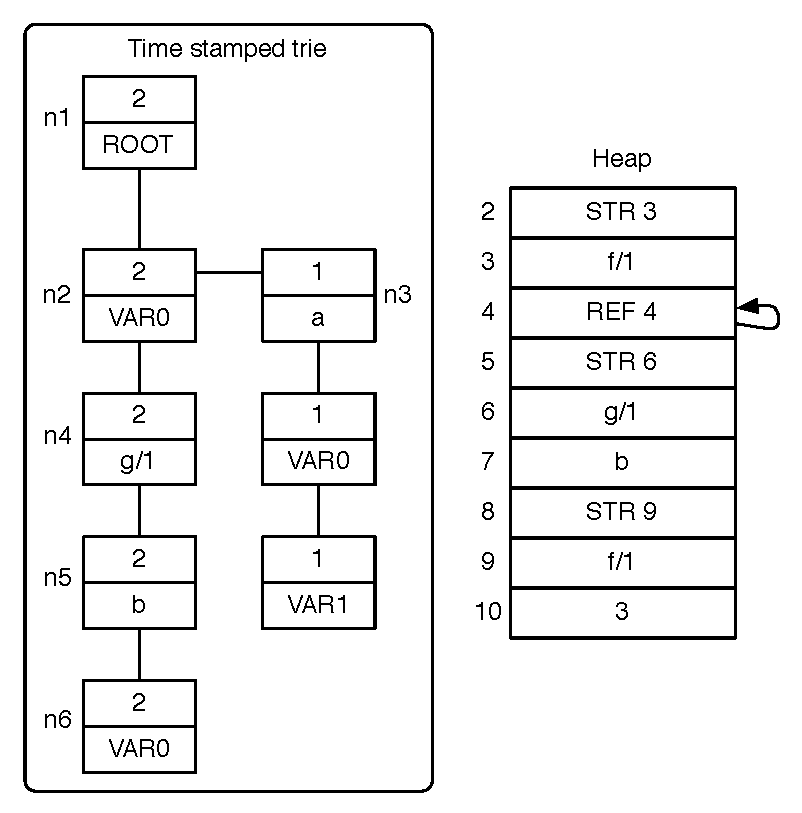
\includegraphics[scale=0.6]{collect_functor.pdf}
  \caption{Example time stamped trie and heap with terms referenced in the answer template.}
  \label{fig:collect_functor}
\end{figure}

At node (a) the term stack contains the full answer template and the variable bindings vector
is empty \ref{fig:collect_functor1}. Only node (b) satisfies the time stamp requirements,
as $2 > 1$.

\begin{figure}[H]
  \centering
    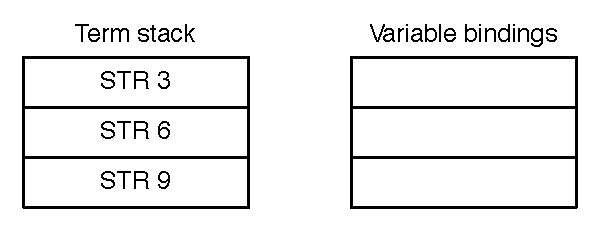
\includegraphics[scale=0.6]{collect_functor1.pdf}
  \caption{Term stack and variable bindings vector at node (a).}
  \label{fig:collect_functor1}
\end{figure}

Node (b) contains a trie variable and the current term is \texttt{STR 3} or \texttt{f(VAR)}.
In this situation, the variable bindings position for \textbf{VAR0} is trailed and bound to \texttt{STR 3}. The data structures configuration is presented in Figure \ref{fig:collect_functor2}.

\begin{figure}[H]
  \centering
    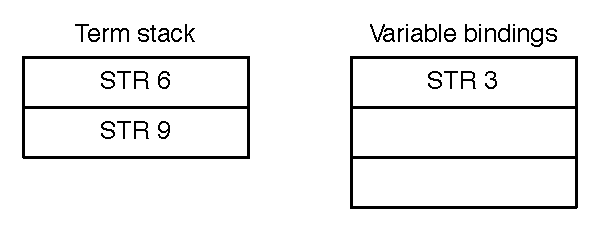
\includegraphics[scale=0.6]{collect_functor2.pdf}
  \caption{Term stack and variable bindings vector at node (b).}
  \label{fig:collect_functor2}
\end{figure}

Node (d) contains the symbol \texttt{g/1} and the current term is \texttt{STR 6}
or \texttt{g(b)}, which matches. The argument \texttt{b} of \texttt{g(b)}
is pushed into the term stack to be processed in the next node (Figure \ref{fig:collect_functor3}).

\begin{figure}[H]
  \centering
    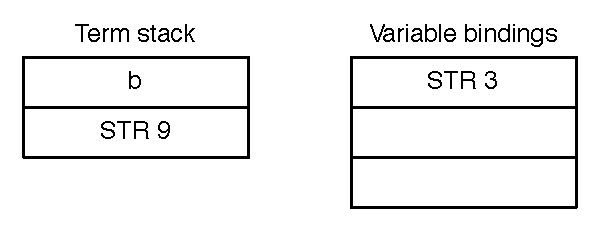
\includegraphics[scale=0.6]{collect_functor3.pdf}
  \caption{Term stack and variable bindings vector at node (d).}
  \label{fig:collect_functor3}
\end{figure}

Node (e) has the symbol \texttt{b} which matches with \texttt{b} from the term stack and
execution proceeds to node (f) (Figure \ref{fig:collect_functor4}).

\begin{figure}[H]
  \centering
    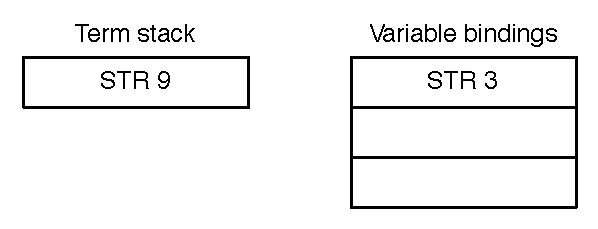
\includegraphics[scale=0.6]{collect_functor4.pdf}
  \caption{Term stack and variable bindings vector at node (e).}
  \label{fig:collect_functor4}
\end{figure}

At (f) we find a trie variable, which, after being dereferenced, contains the
functor \texttt{f(VAR)}. The current term to be unified is \texttt{f(3)}.
In this situation we call \texttt{unify}, which will try to unify both terms.
The unification has the side effect of setting the heap variable cell 4 to \texttt{3}
(Figure \ref{fig:collect_functor5}).
This variable is conditional because it is positioned before the register \texttt{HB},
which given the algorithm design must be greater than 10.

\begin{figure}[H]
  \centering
    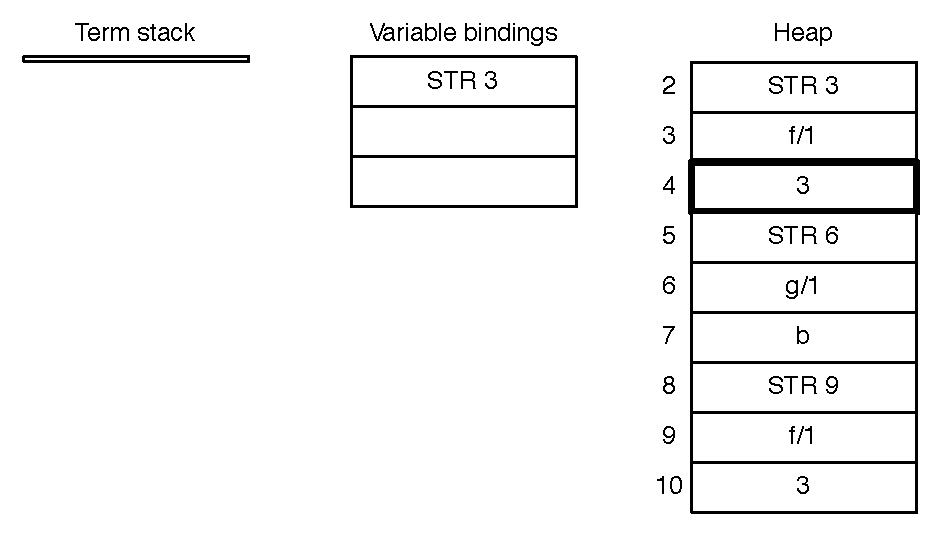
\includegraphics[scale=0.6]{collect_functor5.pdf}
  \caption{Term stack, variable bindings vector and heap at node (f).}
  \label{fig:collect_functor5}
\end{figure}

\subsection{Variable Unification}

Because variables unify with anything, when the top of the term
stack is a variable, the next trie branches only need to be pruned using the time stamp.

Figure \ref{fig:unify_variable} presents the function
\texttt{unify\_variable}. Here, we have three cases:

\begin{enumerate}
  \item The current chain link is an hash table. In this situation we can select the next transitions by using the time stamped index, which can easily prune based on the time stamp;
  \item The current node is inside an hash table, thus is on the time stamped index. The node is matched against the variable and the alternative node is selected by following the index chain links;
  \item Current node is a simple sibling chain. Both the chain and the alternative chain are set by iterating over the node chain, looking for valid time stamps.
\end{enumerate}

Once chains are set, we create a new choice point, run the variable unification algorithm
and proceed into the next trie node.

\begin{figure}[ht]
\begin{Verbatim}
unify_variable(var) {
  if is_hash_table(chain) // case (1)
    index = index_head(chain)
    if timestamp(index) > ts
      chain = node(index)
      alt_chain = next_valid_index(index, ts)
    else backtrack
  else if is_hashed_node(chain) // case (2)
    // can only be here via backtracking
    alt_chain = next_valid_index(get_index(chain), ts)
  else // case (3)
    // simple chain of siblings
    chain = chain_next_valid_node(chain, ts)
    if chain is NULL backtrack
    alt_chain = sibling(chain)
  
  cpstack_push_frame(alt_chain)
  termstacklog_push(var)
  symbol = trie_deref(symbol(chain))
  unifiy_with_variable(var, symbol, chain)
  descend_tst(chain)
}
\end{Verbatim}
\caption{Pseudo-code for \texttt{unify\_variable}.}
\label{fig:unify_variable}
\end{figure}

From the pseudo-code in Figure \ref{fig:unify_with_variable}, variable unification
must consider the following situations:

\begin{itemize}
  \item symbol is a constant: the term variable is bound to the symbol and conditionally trailed.
  \item symbol is a structured term: if the symbol was a trie variable bound to a term then we bind the variable to the heap location; else, we create a new structure (functor or list) on the heap and bind the variable to it, resulting in a term with various heap variables as arguments, which will be pushed into the term stack and will be bound in the next iterations of the algorithm.
  \item symbol is a variable: if the variable is a trie variable, we bind and trail it; if it is an heap variable that was dereferenced from a trie variable using \texttt{trie\_deref}, \texttt{unify} chooses the binding direction, resulting in one of the variables being trailed.
\end{itemize}

\begin{figure}[ht]
\begin{Verbatim}
unify_with_variable(var, symbol, node) {
  if symbol is a constant
    bind_and_conditionally_trail(var, symbol)
  else if symbol is a structured term
    if node symbol is a structured term
      bind_and_conditionally_trail(var, H)
      create_heap_structure(symbol)
      termstack_push_arguments(deref(var))
    else
      // trie variable bound to an heap structure
      bind_and_conditionally_trail(var, symbol)
  else if symbol is a variable
    if symbol is a trie variable
      bind_and_trail(symbol, var)
    else
      // two heap variables
      unify(symbol, var)
  else
    backtrack
}
\end{Verbatim}
\caption{Pseudo-code for \texttt{unify\_with\_variable}.}
\label{fig:unify_with_variable}
\end{figure}

As an example, consider the trie and heap in Figure \ref{fig:collect_variable}.
The input answer template is $\{$\texttt{REF2,REF2,b}$\}$ and the start time stamp is 2.

\begin{figure}[ht]
  \centering
    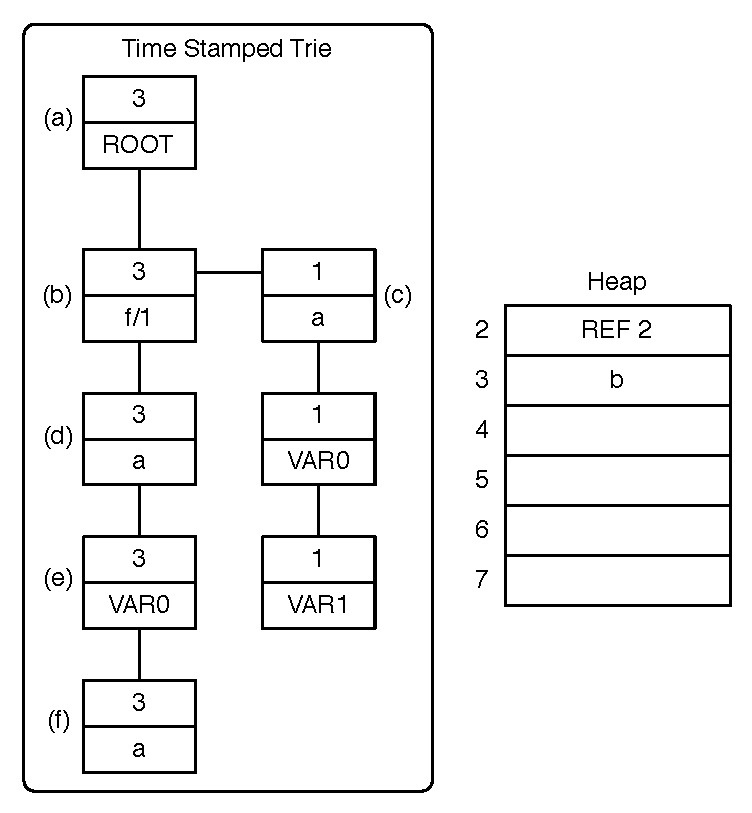
\includegraphics[scale=0.6]{collect_variable.pdf}
  \caption{Example time stamped trie and heap.}
  \label{fig:collect_variable}
\end{figure}

Starting on root node (a), we have the following data structure configuration:

\begin{figure}[H]
  \centering
    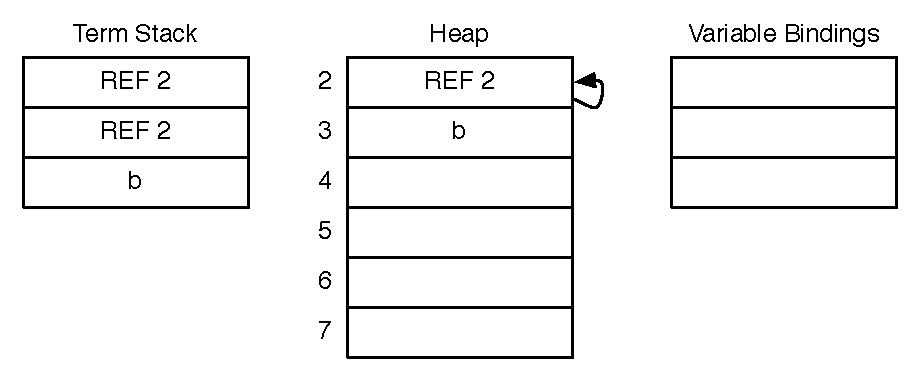
\includegraphics[scale=0.6]{collect_variable1.pdf}
  \caption{At node (a).}
  \label{fig:collect_variable1}
\end{figure}

Node (b) is the only valid transition, with time stamp 3.
The functor \texttt{f/1} is unified against the variable \texttt{REF 2},
which results in the functor \texttt{f/1} being created on the heap
and its argument (\texttt{REF 5}) being pushed into the term stack
(Figure \ref{fig:collect_variable2}).

\begin{figure}[H]
  \centering
    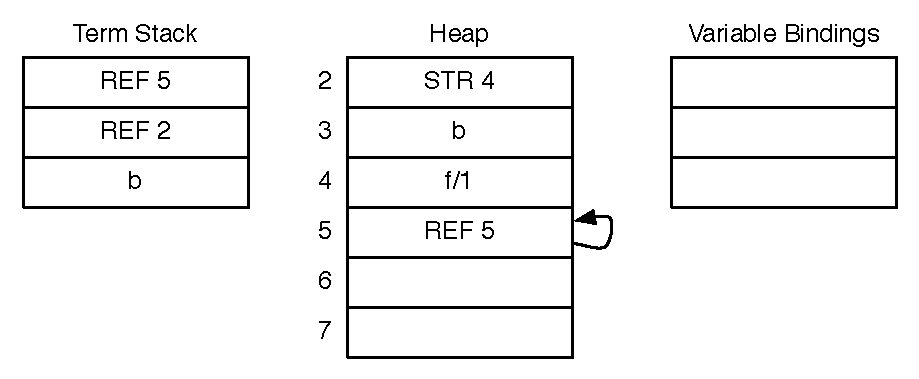
\includegraphics[scale=0.6]{collect_variable2.pdf}
  \caption{After unifying with node (b).}
  \label{fig:collect_variable2}
\end{figure}

The yet unbound functor argument matches atom \texttt{a} in node (d),
resulting in the update of the heap cell 5 (Figure \ref{fig:collect_variable3}).

\begin{figure}[H]
  \centering
    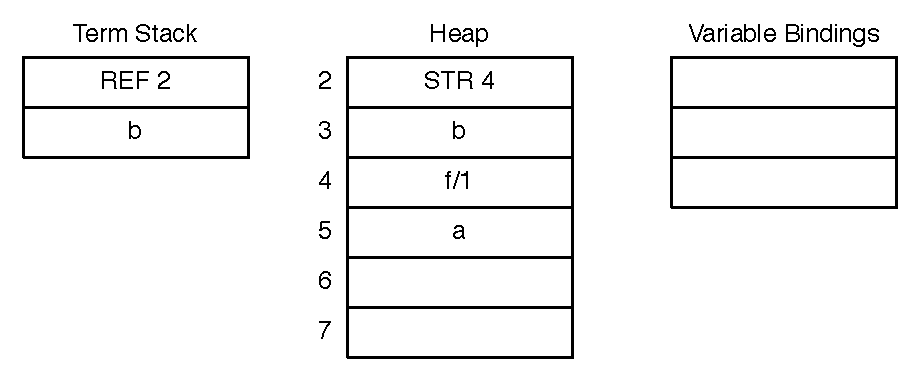
\includegraphics[scale=0.6]{collect_variable3.pdf}
  \caption{After unifying with node (d).}
  \label{fig:collect_variable3}
\end{figure}

Now on the term stack we have \texttt{REF 2}, which dereferences to
a structure on cell 4. On node (e) we have the unbound trie variable
\texttt{VAR0}, which gets bound to \texttt{STR 4} (Figure \ref{fig:collect_variable4}).

\begin{figure}[H]
  \centering
    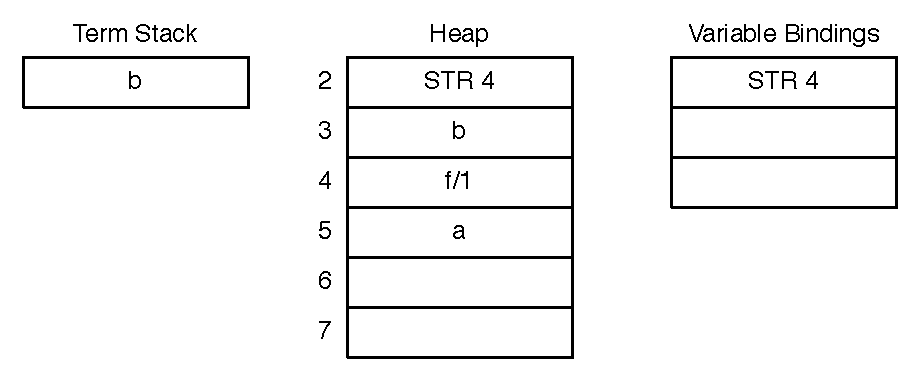
\includegraphics[scale=0.6]{collect_variable4.pdf}
  \caption{After unifying with node (e).}
  \label{fig:collect_variable4}
\end{figure}

Finally, the last term on the term stack is \texttt{b}, which
can not be matched against \texttt{a} on node (f), hence no
relevant answers are found on this trie.

\section{Consuming Answers}

Each consumer subgoal frame stores a linked list with answers that are collected
during evaluation. This list is built incrementally as new answers are generated
for the generator subgoal, which updates the generator time stamp.
Whenever a consumer choice point exhausts the answer list, the retrieval
of relevant answers is attempted so the subgoal frame answer list can be extended.

While the collection of specific answers is done by searching the answer trie
and pruning branches by time stamp and unification failure, it is all done in one
phase. The consumption of a set of answers $S$ is done by consuming one answer $A \in S$
at a time and is completely separated from the collection phase.

Assume we have a trie path from the leaf node $L$ representative of $A$ and
the trie root $R$. Consuming $A$ amounts to unify the symbols on the trie path from $R$ to $L$
to the answer template $AT$ that is built for the consumer choice point. In the end, the variables
on $AT$ are updated so the WAM evaluation branch can proceed with new bindings.

\begin{figure}[H]
  \centering
    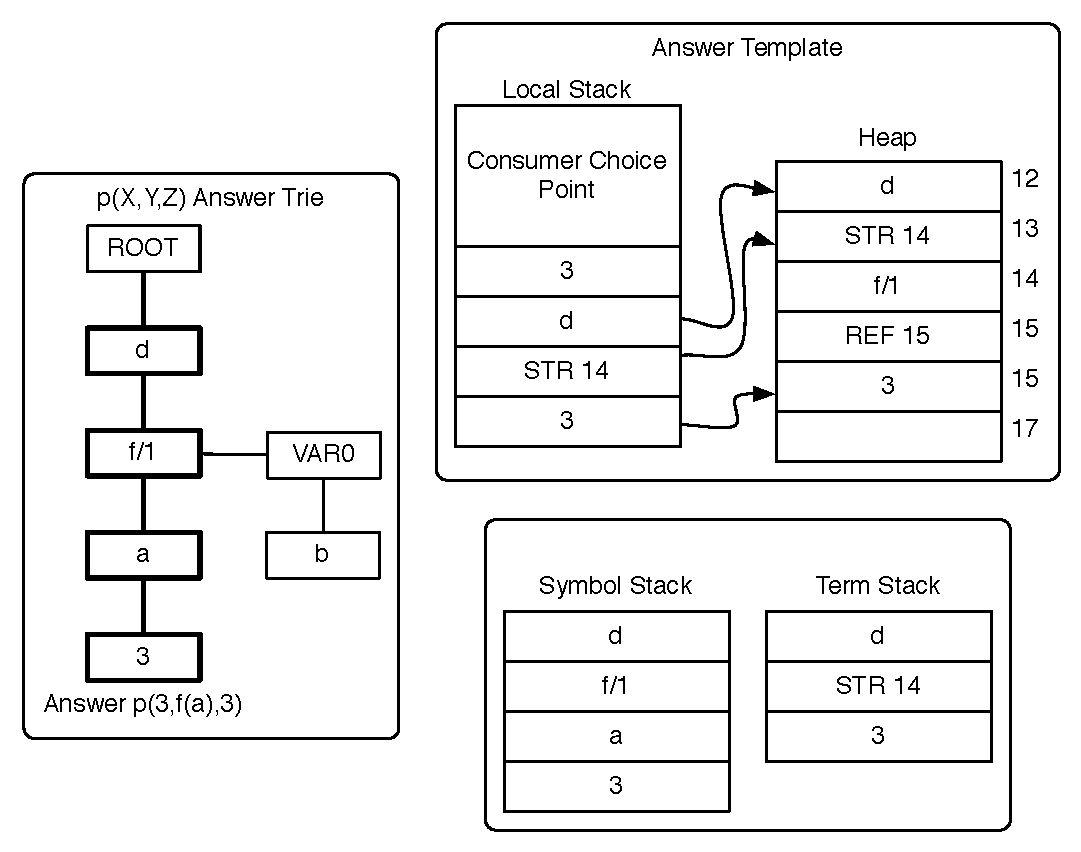
\includegraphics[scale=0.6]{consume_answer.pdf}
  \caption{Data structures related to answer consumption.}
  \label{fig:consume_answer}
\end{figure}

As we are certain that $A$ unifies with $AT$, consumption can be reduced to locating a relevant
answer in a trie with only the answer $A$, no time stamp pruning or backtracking is done.
Implementation wise, we use the term stack that is initially pushed with $AT$
and a symbol stack containing symbols from $R$ to $L$. Then, we proceed by
iteratively popping one term from the term stack and one symbol from the symbol stack
and unifying one against the other.

In Figure \ref{fig:consume_answer} we present the data structures involved in consuming
a subsumptive answer. The subsumptive subgoal is \texttt{p(X,Y,Z)} and the
subsumed subgoal is \texttt{p(d,p(X),3)}. The answer to consume is \texttt{p(d,f(a),3)}.
After the answer is consumed, the subsumed subgoal gets a new answer: \texttt{X = a}.

\section{Compiled Tries}

After an answer trie is completed, it is very common to "compile" the trie,
annotating each trie node with a \textit{trie instruction}. This optimization technique
is called \textit{compiled tries} \cite{RamakrishnanIV-99}.

Compiled tries are based around the observation that all common prefixes of the terms in a trie
are shared during execution of trie instructions. Thus, when backtracking
through the terms of a trie, each transition is taken only once.

\begin{figure}[H]
  \centering
    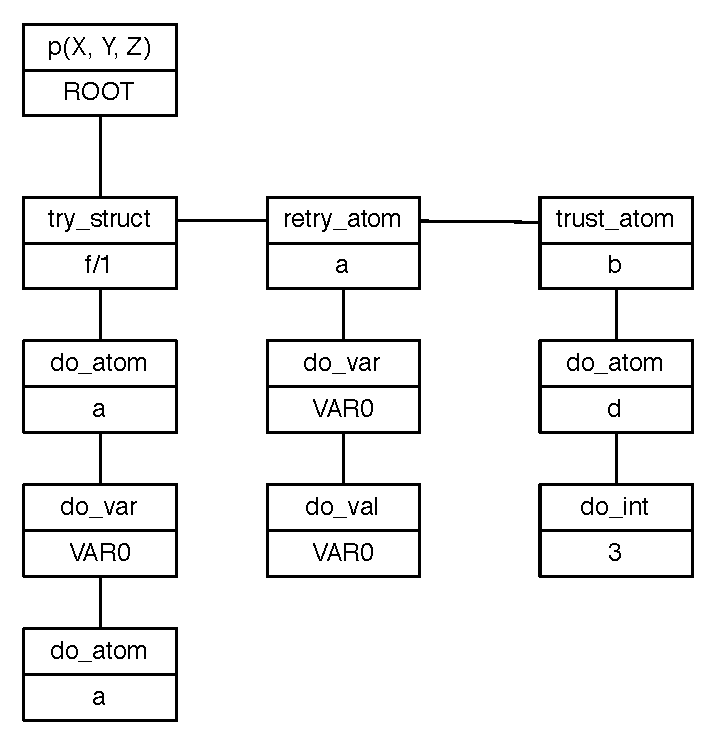
\includegraphics[scale=0.6]{compiled_trie.pdf}
  \caption{A compiled trie for subgoal \texttt{p(X,Y,Z)}.}
  \label{fig:compiled_trie}
\end{figure}

In Figure \ref{fig:compiled_trie} we represent a compiled answer trie for the subgoal
\texttt{p(X,Y,Z)}. Note that each node is extended with an instruction field.
The instruction set follows the standard WAM instruction style with \textit{try},
\textit{retry} and \textit{trust}.
On a sibling chain the leftmost nodes are marked with \textit{try} instructions and middle
nodes with \textit{retry} instructions. Right-most nodes use the \textit{trust} instruction,
while single nodes use the \textit{do} instruction.

A \textit{try} instruction creates a new WAM choice point pointing to the sibling node,
while \textit{retry} instructions change the previous choice point to point to the next sibling node,
thus enabling us to navigate to new trie branches while backtracking. The \textit{trust}
instruction removes the choice point as no more siblings are available. Finally, \textit{do}
instructions do not create choice points as no backtracking options are available.

In a variant tabling engine, each trie instruction just binds each variable on the substitution factor to a term. On structured terms, like functors or lists, the term is first built on the heap and then
bound to the current variable, while the unbound arguments are then passed unto the next trie levels
to be instantiated.

In XSB, time stamped tries are used to evaluate subsumed subgoals while the subsuming subgoal
is incomplete, thus providing incremental retrieving of answers.
When a subgoal $G$ completes, the engine uses the compiled answer trie from $G$
to evaluate a subsumed subgoal $G'$, instead of loading each individual answer.
Using the compiled trie to evaluate $G'$ is thus more efficient, because
each trie path is traversed at most only once. Note that certain paths are pruned when they
are not relevant to $G'$.

Some modifications are thus required to use compiled tries in subsumptive tabling. First,
instead of using the substitution factor when running compiled code, we use the answer template built
on the local stack. Next, each instruction must now do unifications instead of simple bind operations,
because in addition to unbound variables, these instructions can also receive instantiated terms.
Finally, while each instruction succeeds when running with the substitution factor of the generator
subgoal, for subsumed subgoals some instructions can fail, because not every answer will be relevant,
hence will not unify with the answer template. The unification operations done on each trie node
are similar to the unifications done while collecting relevant answers in time stamped tries
(Section \ref{sec:collect}).

\begin{figure}[H]
  \centering
    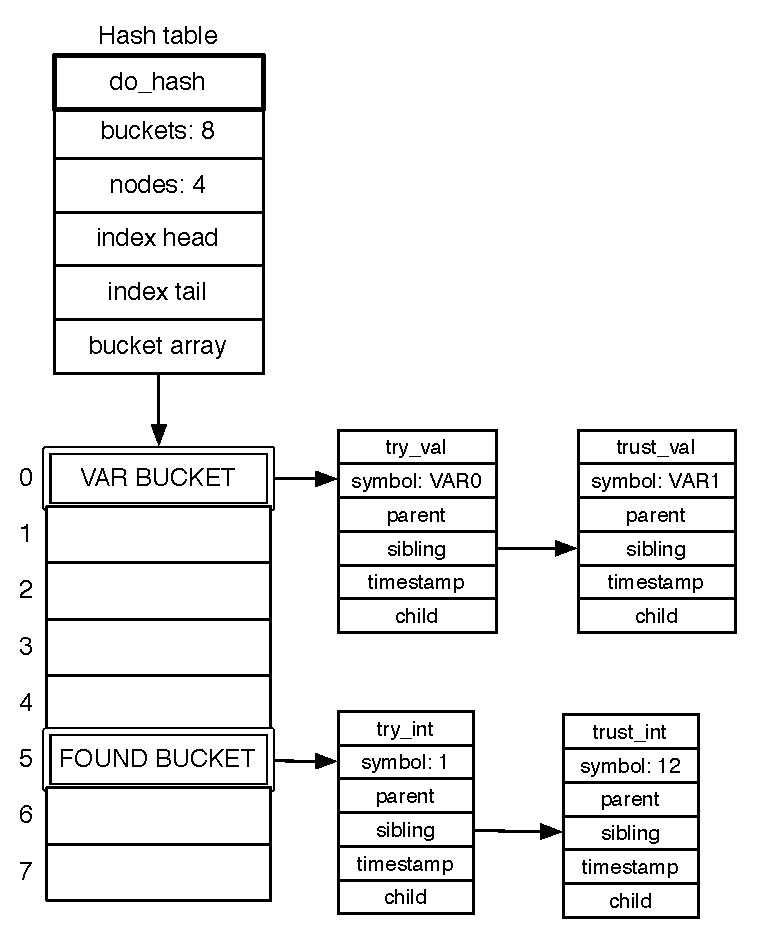
\includegraphics[scale=0.6]{compiled_hash.pdf}
  \caption{Compiled hash table.}
  \label{fig:compiled_hash}
\end{figure}

Variant engines like YapTab collapse each hash table into a chain of nodes before compiling
the trie. While this technique makes sense for a variant engine, in subsumptive engines
having hash tables helps the unification process by enabling fast search of instantiated terms.
Thus, instead of removing hash tables, they are kept and also extended with a new instruction,
\textit{do\_hash} (Figure \ref{fig:compiled_hash}).

When the next term to unify is instantiated we first lookup the bucket for this
term and execute the code of the bucket chain, and optionally we store a choice point that will
execute code from the variable bucket, because variables can unify with any term. If we had
a very long sibling chain, locating a specific term would have a linear time complexity, while
hash tables provide $O(1)$ search complexity.

If the term is a variable, we must visit every trie node in the hash table. This can be done
by storing a choice point where the next hash bucket to execute is stored. If no more
buckets are available, this choice point is removed and the computation fails.

\section{Subsumptive YapTab}

Our first attempt to extend the variant YapTab engine to support call by subsumption
involved importing the subsumption related algorithms and data structures described in
the previous sections from XSB into YapTab. These algorithms were imported as faithful as possible,
hence very little modifications were made as C macros were used to translated the original
code to YapTab. Sections of code specific to XSB or Yap were protected with conditional
compilation, thus enabling both Prolog systems to use the same code.

Other modifications to the following components of YapTab were needed:
tabling instructions, compiled trie instructions, data structures, and algorithms
related to unconsumed answers and consumer detection. This will be explored in the next sections.

We call this modified YapTab engine S1YapTab.

\subsection{Data Structures}

This section describes modifications made to existent data structures and also new 
data structures needed to implement S1YapTab.

\subsubsection{Trie Nodes}

YapTab uses two types of trie nodes: subgoal nodes, for call tries; and answer nodes, for
answer tries. In terms of hash tables, the situation is identical, with subgoal and answer
hash tables. S1YapTab extends the answer and subgoal node with a \texttt{status} field and
creates the time stamped node as an answer node with an extra field: the time stamp.
The \texttt{status} bit field is used to identify the type of trie node, if it is
an hash table, a leaf node or an hashed node.

For hash tables, we extended the answer hash table with
the time stamp indexes to implement the time stamped hash table.
The index data structure was integrally copied from XSB.

\subsubsection{Table Entry}

The table entry contains a bit field called \texttt{mode\_flags} which stores various flags
that change the behavior of tabled predicates. The original YapTab supports the
following mutually exclusive flags: \textbf{batched} / \textbf{local}, the scheduling strategy;
and \textbf{load answers} / \textbf{exec answers}, the later implements the compiled trie optimization, while the first forces the engine to load a completed table by loading answers individually.

Two new mutually exclusive flags were created: \textbf{variant}, which forces the predicate to use variant
tabling and \textbf{subsumptive} to use subsumptive tabling.

\subsubsection{Subgoal Frames}

The subgoal frame structure in YapTab is a main component of the table space.
It contains the fields: \texttt{answer\_trie}, a pointer to the answer trie;
\texttt{state}, the state flag; \texttt{first\_answer} and \texttt{last\_answer}
as the answer return list; \texttt{next}, a pointer to the next executing subgoal;
and \texttt{generator\_cp}, which points to the generator choice point.

Two new kinds of subgoal frame were created: the
\textit{subsumptive producer subgoal frame} and
the \textit{subsumed consumer subgoal frame}.

\begin{figure}[H]
  \centering
    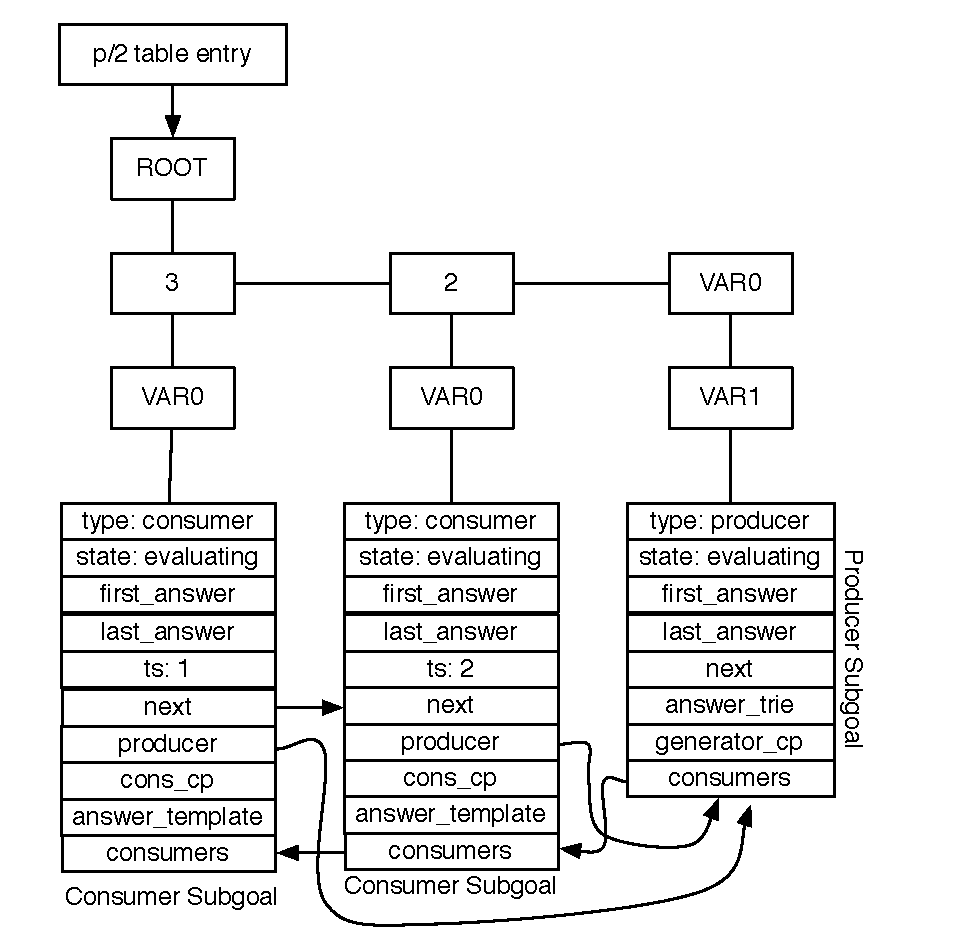
\includegraphics[scale=0.6]{subgoal_frames.pdf}
  \caption{Call trie with producer and consumer subgoal frames}
  \label{fig:subgoal_frames}
\end{figure}

The subsumptive producer subgoal frame extends the original variant subgoal frame
with the field \texttt{consumers}. This field points to a consumer subgoal frame and works
as a chain link to the subsumed subgoal frames of the producer subgoal.

The subsumptive consumer subgoal frame does not extend the variant subgoal frame, because
some variant fields are not needed.
The consumer frame contains the following fields: \texttt{state}, the state of execution;
\texttt{producer}, pointer to the subsumptive producer subgoal frame; \texttt{cons\_cp},
pointer to the first consumer choice point; \texttt{first\_answer} and \texttt{last\_answer},
as the answer return list; \texttt{ts}, the consumer time stamp; \texttt{answer\_template},
a pointer to the answer template built on the heap; and \texttt{consumers},
to link consumer subgoals of the producer subgoal frame.

Each subgoal frame was extended with the \texttt{type} field, which identifies the subgoal frame type.
The variant subgoal now uses an answer return list instead of using the \texttt{child} field of
each trie node to link answers.

Figure \ref{fig:subgoal_frames} illustrates a call trie for the predicate \texttt{p/2}
and the following subgoals: \texttt{p(X,Y)}, a producer subgoal; \texttt{p(2,X)} and
\texttt{p(3,X)} as consumer subgoals. 

\subsection{Tabled Subgoal Call}

The tabled subgoal call operation is one of the four main tabling operations. In YapTab,
if a variant subgoal is already on the table space, a new consumer node is allocated and
and starts to execute \texttt{answer\_resolution}, in order to consume answers. In
the other case, a new generator node is allocated and the tabled subgoal code is executed,
followed by the \texttt{completion} operation, which attempts to complete the SCC if the
generator node is a leader.

\begin{figure}[ht]
\begin{Verbatim}
tabled_subgoal_call(table_entry, arguments) {
  results = subgoal_search(call_trie(table_entry), arguments)
  subgoal_frame = sg_fr(results)
  
  if state(subgoal_frame) == ready
    // new generator
    store_generator_node(table_entry, arguments, subgoal_frame)
    jump_to_predicate_code()
  else if state(subgoal_frame) == evaluating
    // new consumer
    dependency = find_dependency_node(subgoal_frame)
    leader = find_leader_node(subgoal_frame, dependency)
    store_consumer_node(table_entry, subgoal_frame, leader)
    jump_to_answer_resolution()
  else
    // subgoal is completed
    if answer_trie(subgoal_frame) not compiled
      compile_answer_trie(answer_trie(subgoal_frame))
    execute_answer_trie(answer_trie(subgoal_frame))
}
\end{Verbatim}
\caption{Pseudo-code for \texttt{tabled\_subgoal\_call}.}
\label{fig:tabled_subgoal_call}
\end{figure}

Figure \ref{fig:tabled_subgoal_call} presents pseudo-code for the tabled subgoal call.
In the consumer case, we use \texttt{find\_dependency\_node} and \texttt{find\_leader\_node}
to locate the leader node for this consumer. The function \texttt{find\_dependency\_node} simply
returns the choice point of the generator node for this subgoal, while \texttt{find\_leader\_node}
iterates the dependency space between \texttt{dependency} and the new dependency frame for this consumer,
to locate a dependency frame in which the leader is outside this range. If no such dependency frame
exists, the leader node is set as the generator choice point found in \texttt{find\_dependency\_node},
else we use the leader of the dependency frame that satisfied the previous condition. 

S1YapTab extends the tabled subgoal call operation to deal with subsumed subgoals.
If the predicate uses call by subsumption, we use \texttt{subsumptive\_subgoal\_search}
(Figure \ref{fig:subsumptive_subgoal_search}) to look on the call trie for subsuming subgoals.
If no path is found, we insert the subgoal path on the call trie and create a new producer
subgoal frame. If some path is found and the subgoal frame is a producer it can be either
a variant of our subgoal or a more general subgoal. For both cases
we use \texttt{extract\_template\_from\_lookup}, which constructs the right answer template for us.
If the found subgoal frame is a consumer, we must consume from its producer and reconstruct the answer
template by using the producer trie path.
Consumer trie paths are only constructed when the producer subgoal frame is still evaluating.
When the producer is completed, we just execute the compiled trie, so there is no need
to create a consumer subgoal frame.

\begin{figure}[ht]
\begin{Verbatim}
subsumptive_subgoal_search(table_entry, arguments) {
  results = new Results()
  
  (path, leaf) = lookup_subsuming_call(call_trie(table_entry), arguments)
  
  if path == NO_PATH
    variant_found(results) = FALSE
    leaf(results) = insert_with_variant_continuation(call_trie)
    // create a variant answer template
    answer_template(results) = extract_template_from_insertion(local_stack)
    sg_fr(results) = create_producer_subgoal_frame(leaf(results))
  else
    // new consumer
    subsumer = subgoal_frame(leaf)
    
    if type(subsumer) == producer
      answer_template(results) = extract_template_from_lookup(local_stack)
    else
      subsumer = producer(subsumer)
      answer_template(results) = reconstruct_template_for_producer(subsumer, local_stack)
    
    variant_found(results) = (path_type == VARIANT_PATH)
    
    if path_type != VARIANT_PATH && state(subsumer) == evaluating
      // create variant path
      leaf(results) = insert_with_variant_continuation(call_trie)
      sg_fr(results) = create_new_consumer_subgoal(leaf(results), subsumer)
      copy_answer_template_to_heap(answer_template(results))
    else
      sg_fr(results) = subsumer
  
  return results
}
\end{Verbatim}
\caption{Pseudo-code for \texttt{subsumptive\_subgoal\_search}.}
\label{fig:subsumptive_subgoal_search}
\end{figure}

When a consumer subgoal frame is created we make a structural copy of the answer template
into the heap. This copy of the answer template will be used as an argument
to the algorithm that collects relevant answers from the producer answer trie.
Each consumer subgoal frame has just one copy of the answer template on the heap,
while each consumer node uses its own answer template built on the stack to
consume answers, because it references variables
and terms from the arguments.

The field \texttt{cons\_cp} of the consumer subgoal frame is set to point to the first call
of the consumer subgoal and will be used access the value of \texttt{H} stored on the choice point.
This value of \texttt{H} points to the top of the heap during the choice point creation which corresponds
to the answer template copied before. The field \texttt{answer\_template} points to this \texttt{H}
and is used to avoid accessing the choice point, thus it must be recalculated during garbage collection.

This differs from XSB \cite{XXX} where a non-structural copy of the answer template is built on the heap for each
consumer node, but whenever the need to collect relevant answers arises, we must reconstitute the
environment of the consumer to ensure that the answer template is valid, which involves using the trail
to unbind and/or rebind variables. Our approach has the disadvantage of making structural copies,
but only one copy is done and there is no need to invoke the algorithm
within the environment of the subsumed call.

\begin{figure}[ht]
\begin{Verbatim}
tabled_subgoal_call(table_entry, arguments) {
  results = subgoal_search(call_trie(table_entry), arguments)
  subgoal_frame = sg_fr(results)
  
  if is_new_generator_call(results)
    store_generator_node(table_entry, arguments, subgoal_frame)
    jump_to_predicate_code()
  else if is_new_consumer_call(results)
    dependency = find_dependency_node(subgoal_frame)
    leader = find_leader_node(subgoal_frame, dependency)
    store_consumer_node(table_entry, subgoal_frame, leader)
    if type(subgoal_frame) == consumer and state(subgoal_frame) == ready
      cons_cp(subgoal_frame) = B
      recompute_answer_template(subgoal_frame)
    jump_to_answer_resolution()
  else
    // subgoal is completed
    if answer_trie(subgoal_frame) not compiled
      compile_answer_trie(answer_trie(subgoal_frame))
    execute_answer_trie(answer_trie(subgoal_frame))
}
\end{Verbatim}
\caption{Pseudo-code for the new \texttt{tabled\_subgoal\_call}.}
\label{fig:tabled_subgoal_call_new}
\end{figure}

Other modifications were applied in order to abstract some details about
variant and subsumptive tabling (Figure \ref{fig:tabled_subgoal_call_new}).
The function \texttt{is\_new\_generator\_call} inspects the return value
of \texttt{subgoal\_search} in order to tell if a new generator node must be allocated.
For call subsumption, a new generator is called whenever a variant subgoal is not found
on the trie and the resulting subgoal frame is a producer.
The function \texttt{is\_new\_consumer\_call} knows a new consumer node must be
allocated when:

\begin{enumerate}
  \item The subgoal frame is variant or producer and is currently being evaluated;
  \item The subgoal frame is consumer and the producer subgoal is still evaluating.
\end{enumerate}

Another important change involves calculating the leader node of a subsumptive consumer node.
Surprisingly, only the algorithm to find the dependency node must be altered, as
the dependency node of a subsumptive consumer is the generator choice point of
the producer subgoal frame (Figure \ref{fig:find_dependency_node}).  

\begin{figure}[ht]
\begin{Verbatim}
find_dependency_node(subgoal_frame) {
  if type(subgoal_frame) == variant or type(subgoal_frame) == producer
    return generator_cp(subgoal_frame)
  else
    return generator_cp(producer(subgoal_frame))
}
\end{Verbatim}
\caption{Pseudo-code for the new \texttt{find\_dependency\_node}.}
\label{fig:find_dependency_node}
\end{figure}

\subsection{Answer Resolution and Completion}

The tabling operations answer resolution and completion both check if a
given consumer node has unconsumed answers. The completion operation
iterates over the dependency space to look for consumer nodes with unconsumed
answers and the answer resolution operation attempts to consume the next answer
of a consumer and also iterates over the dependency space in order to run the completion algorithm.

In order to abstract away if a consumer node has answers to consume,
we created a function that distinguishes between both variant and subsumptive cases
(Figure \ref{fig:get_next_answer_continuation}).
The function accepts a dependency frame (note that there is a dependency frame for
each consumer node) and returns an answer continuation, which contains the answer
to consume and contains enough state to retrieve the next available answer continuation, if any.
An answer continuation is represented by a pointer to a linked list with two fields:
\texttt{answer} and \texttt{next}, which points to the next element of the list.

\begin{figure}[ht]
\begin{Verbatim}
get_next_answer_continuation(dependency_frame) {
  sg_fr = depfr_sg_fr(dependency_frame)
  last_continuation = depfr_last(dependency_frame)
  next_continuation = continuation_next(last_continuation)
  
  if type(sg_fr) == variant or type(sg_fr) == producer
    return next_continuation
  
  if next_continuation is not NULL
    return next
  
  // must collect new available answers, if any
  consumer_ts = timestamp(sg_fr)
  producer = producer(sg_fr)
  producer_ts = timestamp(answer_trie(producer))
      
  if(producer_ts == consumer_ts)
    return NULL
        
  // collect answers
  answer_list = tst_collect_relevant_answers(answer_trie(producer),
        consumer_ts, answer_template(sg_fr))
  timestamp(sg_fr) = producer_ts
      
  if answer_list is not NULL
    append_return_list(sg_fr, answer_list)
      
  return answer_list
}
\end{Verbatim}
\caption{Pseudo-code for \texttt{get\_next\_answer\_continuation}.}
\label{fig:get_next_answer_continuation}
\end{figure}

With subsumptive consumer nodes we first verify if the answer return list of the
consumer subgoal frame contains more answers from the saved continuation. If there is
any, we return the next answer from this list and consume it. If the list has no more answers,
we inspect if the consumer time stamp is equal to the producer time stamp, which means
that no new answers were generated for the general subgoal. In the other hand, if new
answers are available, we run \texttt{tst\_collect\_relevant\_answers} to collect any
relevant answers for this consumer that can be appended unto the answer return list
and returned for consumption.
In any case, the time stamp of the consumer is thus updated to avoid collecting
repeated answers in future iterations. Remember that once a single consumer node
collects newer answers, every consumer node of a subsumptive subgoal will see them, thus
enabling sharing of answers among the consumer nodes.

The dependency frame data structure was extended with the \texttt{sg\_fr} field, so it could
be possible to run this algorithm and the completion algorithm presented in the next section.

\begin{figure}[ht]
\begin{Verbatim}
completion(generator) {
  if G is the current leader node
    df = TOP_DF
    while depfr_cons_cp(df) is younger than G {
      cont = get_next_answer_continuation(dep_fr)
      if cont
        // unconsumed answers
        depfr_back_cp(df) = G
        C = depfr_cons_cp(df)
        restore_bindings(CP_TR(G), CP_TR(C))
        goto answer_resolution(C)
      df = depfr_next(df)
    }
    perform_completion()
    adjust_freeze_registers()
  backtrack_to(CP_B(G))
}
\end{Verbatim}
\caption{Pseudo-code for the updated \texttt{completion} operation.}
\label{fig:completion_operation}
\end{figure}

Figure \ref{fig:completion_operation} presents the updated \texttt{completion} operation,
using the devised abstractions.

\subsection{Completion}

Once a generator node completes we must mark each subgoal that appears under the SCC as \textit{complete}.
Hence, some modifications must be made to complete subsumptive consumer subgoal frames.

In YapTab each variant subgoal frame is chained in a linked list during execution. The top of this list
can be accessed by using the \texttt{LOCAL\_top\_sg\_fr} and completion is done by iterating this list until
the target subgoal frame is reached. The dependency frames that are younger than the completion point
are also iterated and freed. 

Subsumptive consumer subgoal frames are easily accessible by using the \texttt{sg\_fr} field in the dependency frames.
Thus, to complete these subgoals, while freeing the dependency frames we check if the subgoal is not complete and a
subsumptive consumer.

Some data structures, like the time stamp indexes, are deleted during completion from the
subsumptive producer subgoal frames.

\begin{figure}[H]
  \centering
    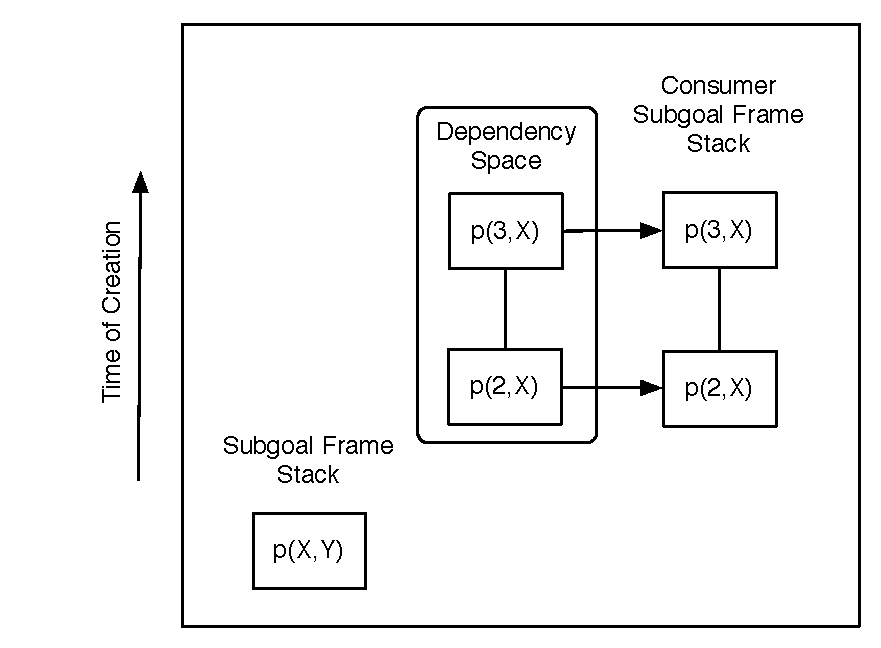
\includegraphics[scale=0.6]{completion_space.pdf}
  \caption{Subsumptive producer and consumers before completion.}
  \label{fig:completion_space}
\end{figure}

\subsection{Compiled Tries}

\section{Results}
